% Load document class

% possible options: color/nocolor, english/german, threecolumn
% default: color, english
\documentclass[english, leagacyboxes, nologo]{latex4ei/latex4ei_sheet}

\usepackage{upquote}
\usepackage{latex4ei/latex4ei_colors}
\usepackage{float}
\usepackage{graphicx}

\begin{document}
\title{Network Security}
\author{Stephan Dollberg, Martin Zellner, Nelly Afonso, Pierre Dumont and Lucas Vandroux}
\myemail{lucas.vandroux@gmail.com}      % optional, delete if unchanged
\mywebsite{www.latex4ei.de}     % optional, delete if unchanged
\maketitle
\section{Introduction}

  \sectionbox{
  \subsection{Security Trends}
    Network security is an issue since \emph{critical infrastructures} in the open systems with a growing user base (\ra \emph{increasing risk}) are threatened by \emph{organized crime}.
  }
  \sectionbox{
  \subsection{Security Threats}
    \textbf{Asymmetric Threat:} Defenders must protect against all exploits on all systems but attackers can attack only a few.

    \textbf{Attacker Motivation:} Ego, Revenge, Destruction, Criminal intend, Acquisition of resources, Acquisition of sensitive information
  }
  \sectionbox{
  \subsection{Security Concepts}
    \textbf{CIA Triad}
    \begin{itemize}
      \item Confidentiality (prevention of unauthorized disclosure)
      \item Integrity (prevention of unauthorized modification or deletion)
      \item Availability (prevention of unauthorized withholding)
     \end{itemize}

     Also: Authenticity, Accountability(Responsability), Nonrepudiation (Can't deny), Privacy

     \textbf{Passive attacks:} Confidentiality (Eavesdropping, Content compromise, Traffic analysis)

     \textbf{Active attacks:} Availability (Denial of service), Integrity and Authenticity (Modification, Replay, Fabrication)

     \textbf{Secure Channel:} secure = authentic (of the sender) and confidential (no eavesdropping)

     \textbf{Security on OSI-Layers:} Physical (Link encryption), Network (IPSEC), Transport (SSL), Application (SSH)
   }

   \sectionbox{
   \subsection{OSI (Open Systems Interconnection)}
     \begin{tabular}{ | l | l | l |}
       \hline
       OSI Model & Data Seq. & Protocols + Port\\
       \hline
       \cellcolor{notsodarkblue} Application & Message & FTP 20-21, SSH 22, Telnet 23\\
       \cline{1-1}
       \cellcolor{notsodarkblue} Presentation* & & SMTP 25, HTTP/s 80/443\\
       \cline{1-1}
      \cellcolor{notsodarkblue} Session* & & DHCP, NTP, BGP 179, TLS\\
       \hline
       \cellcolor{notsodarkgreen} Transport & Segment & TCP, UDP\\
       \hline
       \cellcolor{notsodarkpurple} Network & Datagram & IP, IPSec, ICMP, IGMP, OpenVPN\\
       \hline
       \cellcolor{notsodarkred} Data Link* & Frames & Ethernet, ARP\\
       \cline{1-2}
       \cellcolor{notsodarkred} Physical  & Bit Stream & 802.11 (WiFi)\\
       \hline
     \end{tabular}\\
     * \textit{Don't exist in \textbf{TCP/IP Model:}}  \textcolor{notsodarkpurple}{Internet Layer} \textcolor{notsodarkred}{Link Layer}
   }

  \sectionbox{
  \subsection{ARP (Address Resolution Protocol)}
    Use to find MAC add. corresponding to IP add. in LAN $\ra$ request is broadcast MAC add. (FF:FF:FF:FF:FF:FF) $\ra$ answer store in ARP cache

    \textbf{ARP Spoofing}(=ARP cache poisoning/ARP poison routing) $\ra$ possible because ARP stateless + no authentication $\Ra$ MitM + DOS attacks

    $\Ra$ \underline{Defense}: static ARP entries +/ certify/cross-check ARP answers

    \textbf{Cache lifetime}: a few 10 seconds (avoiding frequent ARP requests)

    \textbf{Switch}: extends LAN (layer 2) $\ra$ forward Frames

    \textbf{Router}: forward IP datagram (layer 3)

    \textbf{Note:} ARP req. + MAC broadcasts don't go across routers
  }

 \sectionbox {
 \subsection{HTTP (Hypertext Transfer Protocol)}
   \begin{itemize}
     \item Stateless protocol (Server doesn't know which client connects again)
     \item Status Code : 1xx info, 2xx success, 3xx redirection, 4xx client error, 5xx server error
     \item HTTP\_REFERER : header field, identifies address of webpage  that linked to the resource being requested (due to proxy not always set)
     \item HTTP methods : GET, POST, PUT, DELETE, HEAD
     \item HTTP cookie : name$\leftrightarrow$value (expiration date, stored by client)
     \begin{itemize}
       \item Use for session management, secure cookie (HTTPS only)
     \end{itemize}
   \end{itemize}
 }


\section{(In)securtity, Risk \& Vulnerability Lifecycle}

  \sectionbox{
  \subsection{(In)security Landscape}
    General: complexity is bad (but increases fast)

    Security of a system := Security of its weakest link
  }
  \sectionbox{
  \subsection{Vulnerablity Lifecycle}
    \textbf{Security vulnerability}: A weakness in a system allowing an attacker to violate the confidentiality, integrity, availability of the system or the data and applications it hosts disagreement on what is a vulnerability possible (it's a a feature not a vulnerability)

    \textbf{CVE}: Standard names for all publicly known vulnerabilities and security exposures. De facto standard. (Form: \emph{CVE-Year-AnyDigits})

    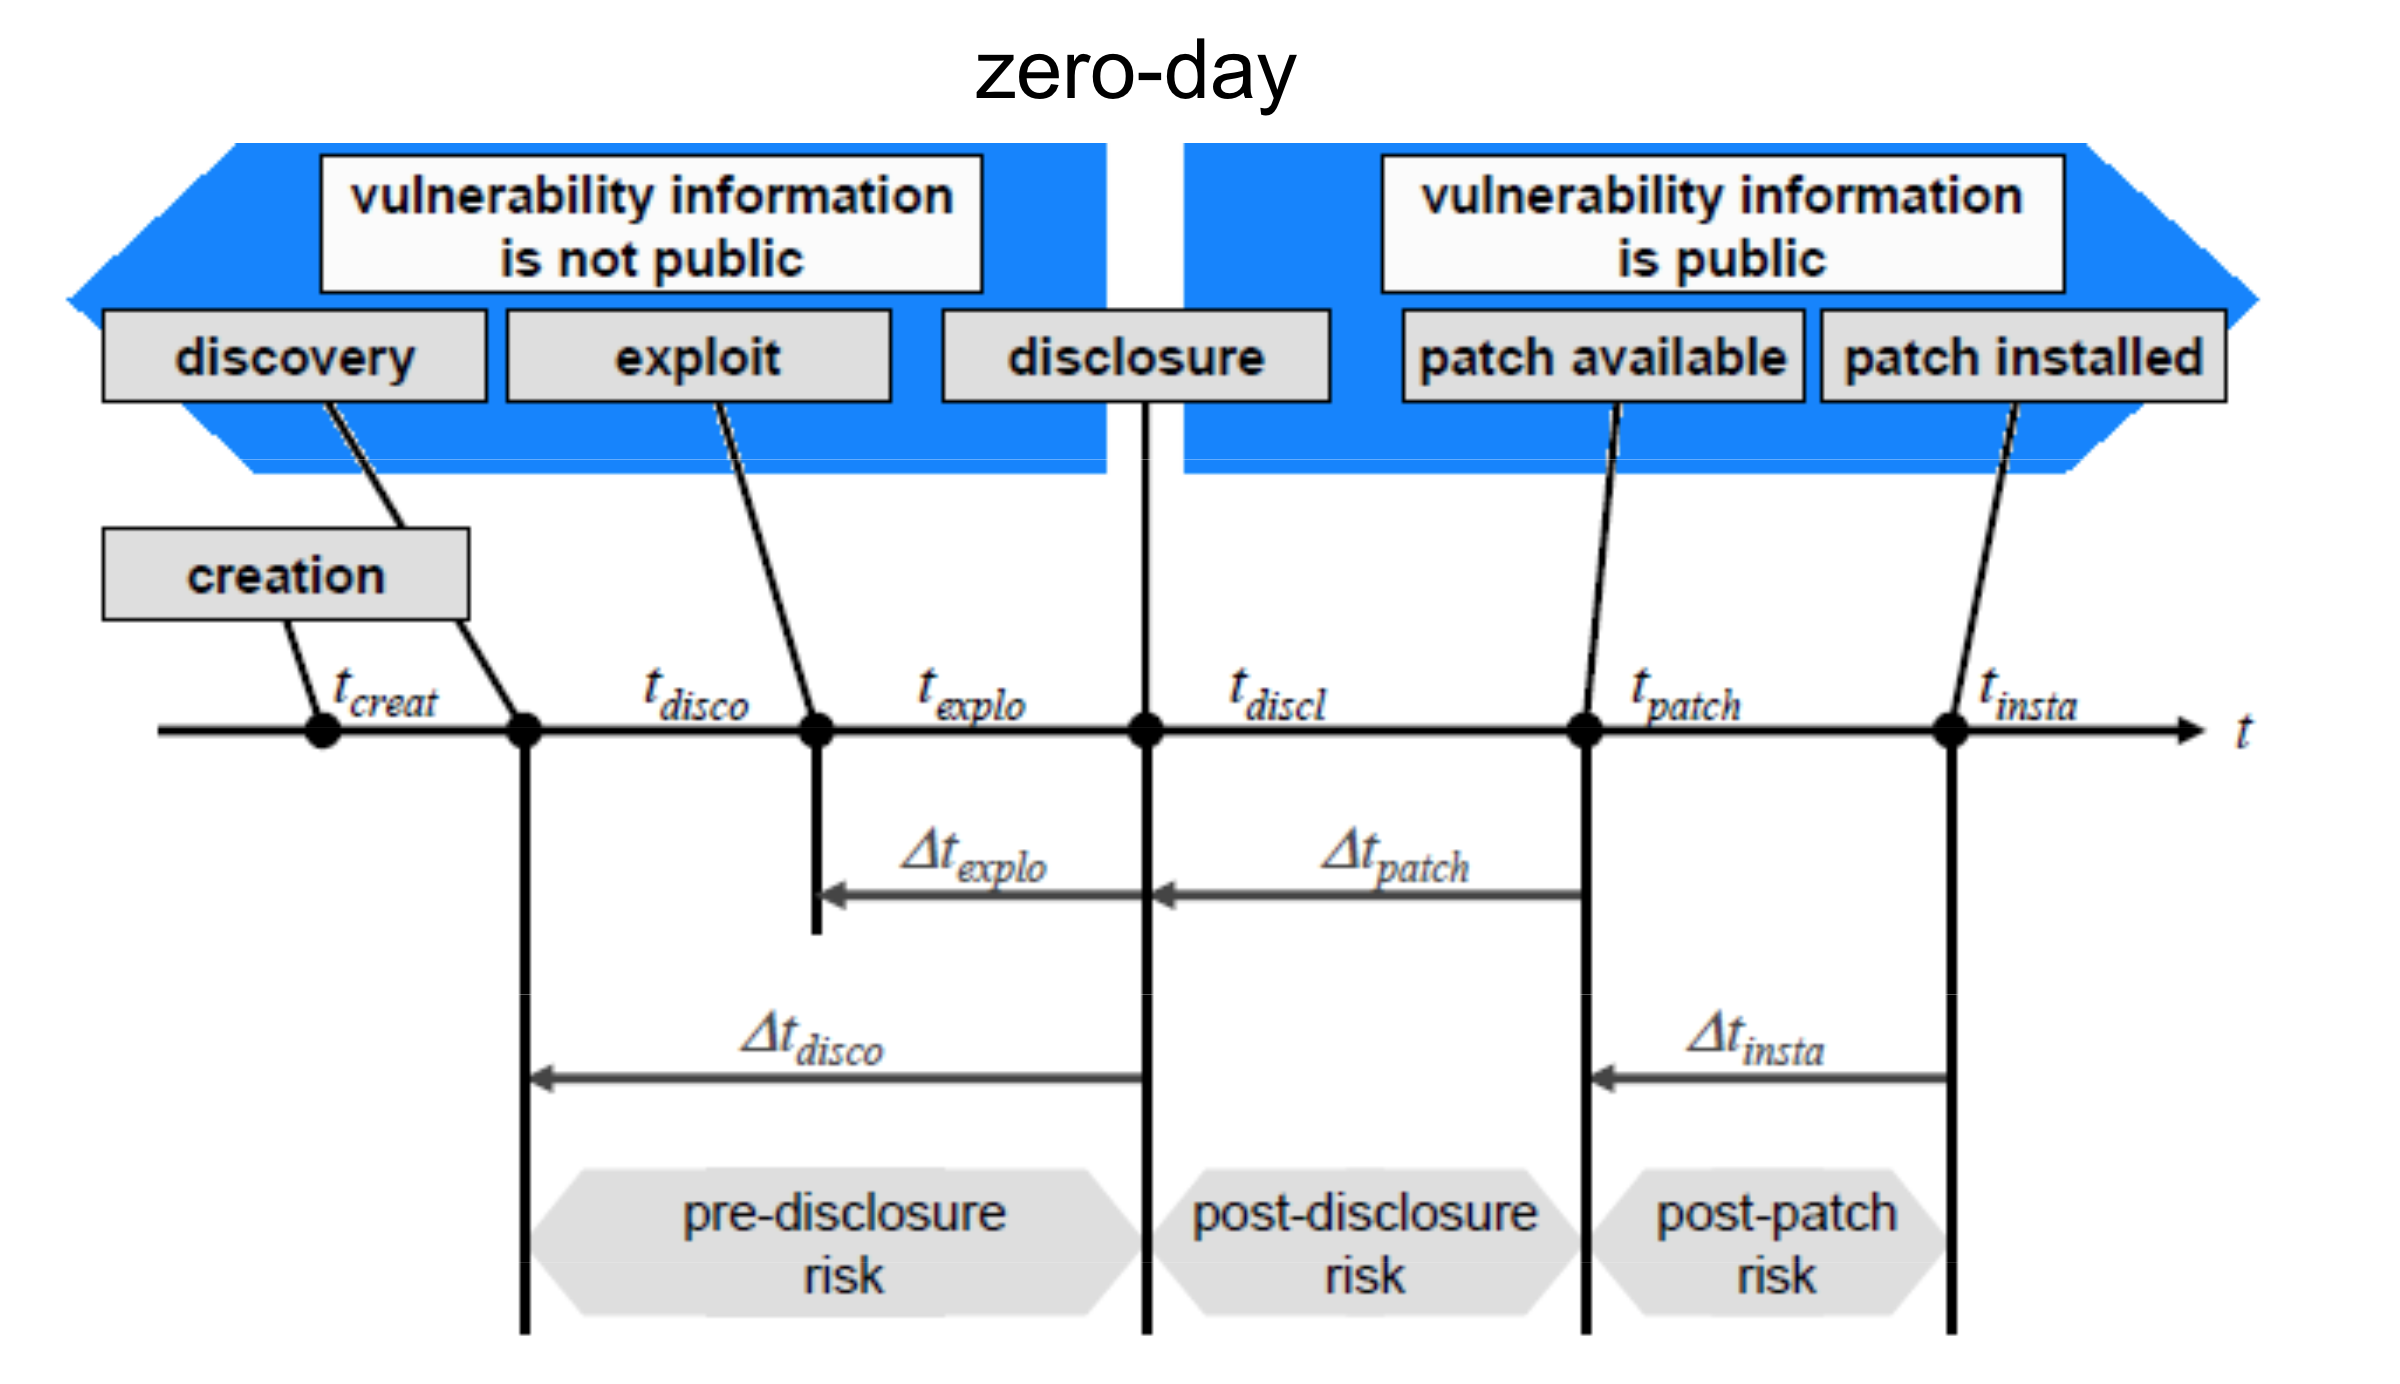
\includegraphics[width=\columnwidth]{img/VUL-LC.png}

    \textbf{Zero-day} Date when the vulnerability becomes known by the public

    \textbf{Zero-day-exploit} Attack that exploits a previously unknown vulnerability

    \textbf{Numbers:}\\
    50 \% of vulnerabilities known to insiders 30 or more days before disclosure (less-than-zero-day)

    At disclosure (zero-day):  $\approx 50 \%$ unpatched + $\approx 80 \%$ exploits available

    Exploit availability jumps from 15\% to 80\% after disclosure

    A month after disclosure: $\approx 30 \%$ unpatched
  }

  % Move the numbers in the section below
  \sectionbox{
  \subsection{Dynamics of (In) Security}
    \begin{itemize}
      \item extremely high dynamics around the disclosure
      \item exploit availability stays higher than the patch availability
      \item insiders: may know undisclosed vulnerabilities
    \end{itemize}

    \textbf{Gap of insecurity:} Difference between the exploit and patch (the bad a consistently faster than the good)

    \textbf{Security is slow:} Many vulnerabilities are unpatched even 100 days after disclosure.

    \textbf{Market for new vulnerabilities:} ZeroDayInitiative and Black Market, pricing from 1000 to more than 200 000 USD
  }

  \sectionbox{
  \subsection{Risk Management}
    There is no such thing as absolute security

    Trade-Off between security and financial, social, functional, \ldots

    \subsubsection{Risk analysis}
    \begin{itemize}
      \item What assets are we trying to protect?
      \item what are the risk to those assets?
      \item How well does the security solution mitigate those risks?
      \item What other risks does the security solution cause?
      \item What costs and trade-offs does the security solution impose?
    \end{itemize}
    \ra Is the trade-off worth if?

    \subsubsection{Risk management}
    Security is relative \Ra manage risks

    \underline{Options}: avoid, decrease, transfer, accept risk

    \underline{Business sense}: risk $<$ opportunity
  }


\section{Identity and Authentication}

  \sectionbox{
  \subsection{Identity and Identity Theft}
    \textbf{Authentication:} Authentication is the process of verifying an identity claim of an entity. It binds the principal to an identity

    \textbf{Authentication Criteria:}
    \begin{itemize}
      \item Something an entity knows (e.g. password, PIN)
      \item Something an entity has (e.g. key, card)
      \item Something an entity is (e.g. biometric characteristic)
      \item rarely used: location, ability
    \end{itemize}

    \textbf{Types of ID Theft}
    \begin{itemize}
      \item \underline{Financial Identity Theft}: using someone else credit card, using another's name and SSN to obtain goods and services (e.g. open a bank account, purchase on invoice)
      \item \underline{Criminal Identity Theft}: posing as another when apprehended for a crime
      \item \underline{Identity Cloning}: using another's information to assume his or her
identity in daily life
      \item \underline{Business/Commercial Identity Theft}: using another's business name to obtain credit
    \end{itemize}

    \textbf{Weak authentication:} checking only one authentication criteria

    \textbf{Strong authentication:} checking two or more authentication criteria

    \textbf{FIDO (Fast IDentity Online) Alliance}

    Non-profit organization addressing:
    \begin{itemize}
      \item lack of interoperability among strong authentication devices
      \item problems users face with creating and remembering multiple usernames and passwords
    \end{itemize}
    Members : Google, Microsoft, PayPal, Samsung, intel, RSA etc
  }

  \subsection{Authentication Protocols}

    \sectionbox{
    \subsubsection{OAuth}
      Allows sharing of private resources across web sites.

      To access the data, tokens are used instead of credentials.

      \textbf{Limitation:} possibility of impersonation of resource owner (via phishing)

      \textbf{Many eggs in one basket} if central account becomes hacked, or you simply choose to close the account, then the serious repercussions are felt across several sites instead of just one.

      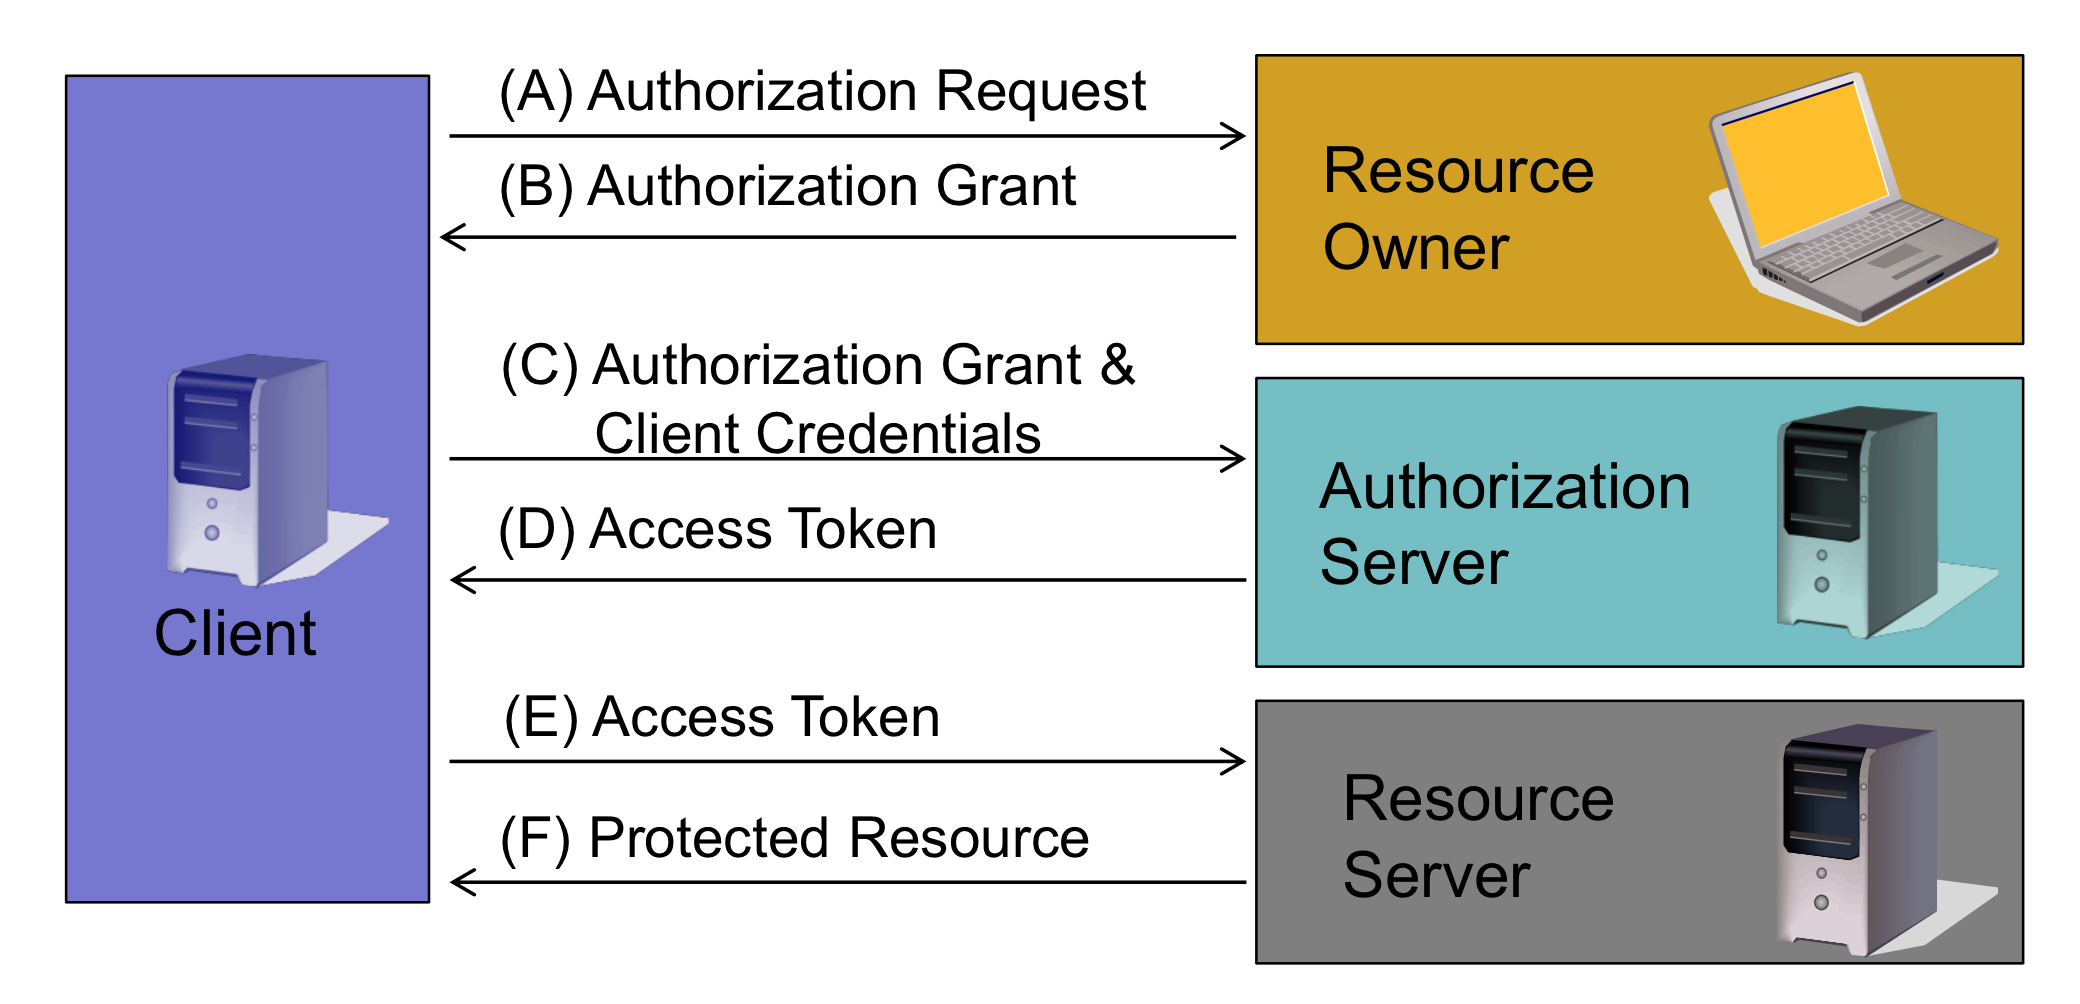
\includegraphics[width=\columnwidth]{img/OAuth.png}

      \textbf{Resource Owner}: Entity capable of granting access to a protected resource. When resource owner is a person, it is referred to as an end-user.

      \textbf{Client}: An application making protected resource requests on behalf of the resource owner and with its authorization (e.g. a web browser for a printing service webpage).

      \textbf{Authorization server}: The server issuing access tokens to the client after successfully authenticating the resource owner and obtaining authorization

      \textbf{Resource server}: Server hosting the protected resources, capable of accepting and responding to protected resource requests using access tokens.
    }

    \sectionbox{
    \subsubsection{OpenID}
      Standard for decentralized user authentication:
      use existing account to sign in to multiple websites without creating a new password

      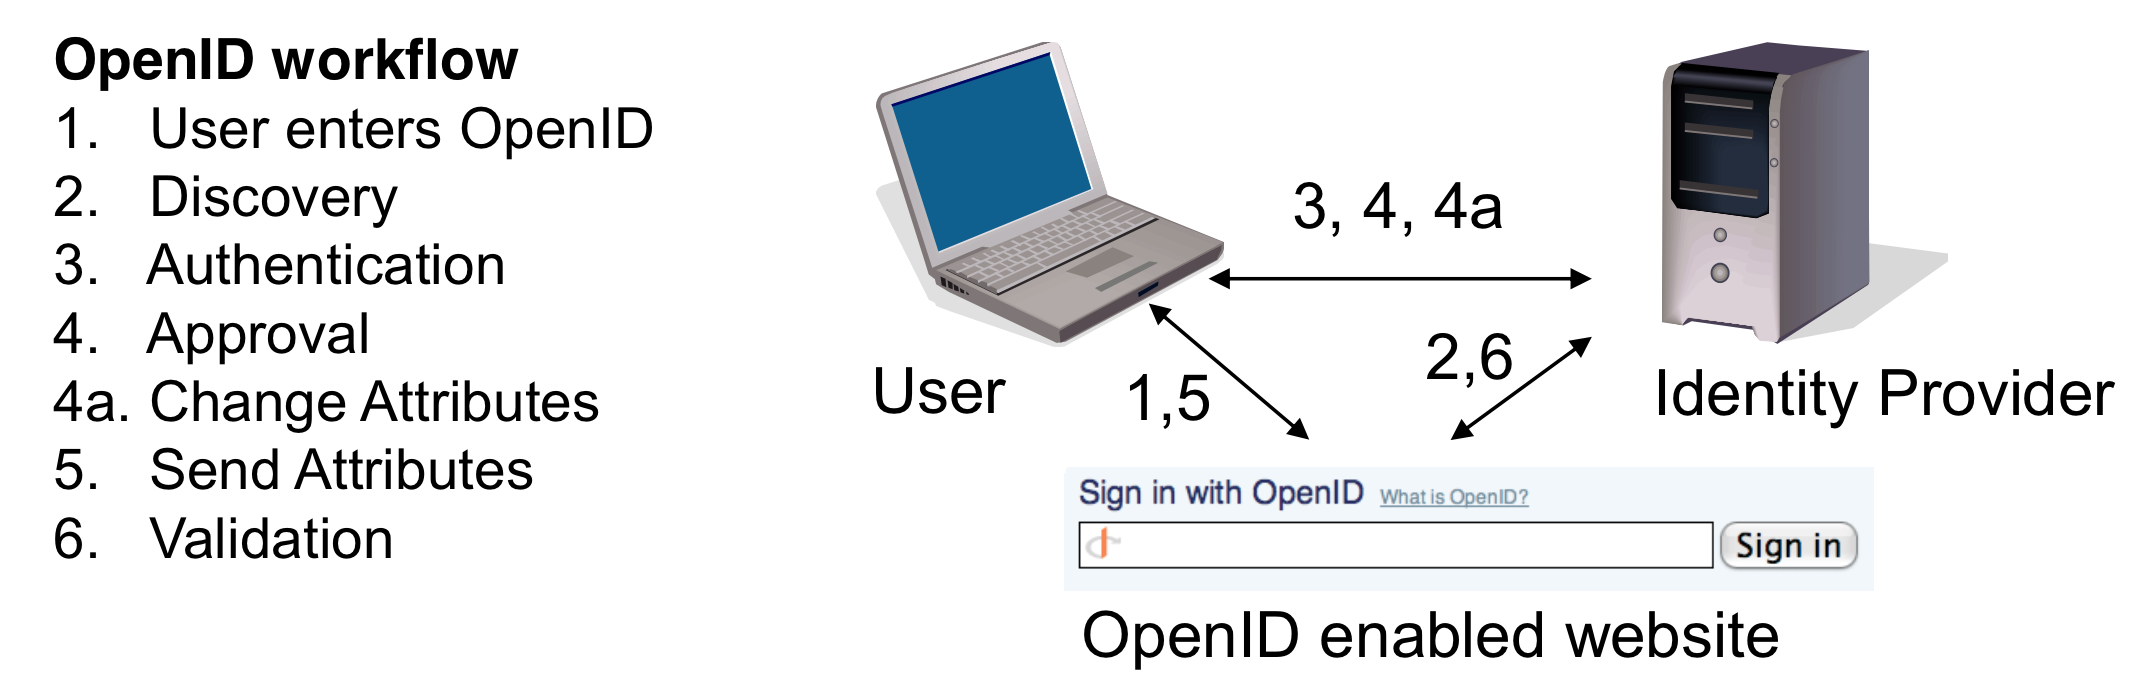
\includegraphics[width=\columnwidth]{img/OpenID.png}
      \textbf{Need to trust the identity provider.}
    }

    \sectionbox{
    \subsubsection{3D Secure}
      A protocol used widely to authenticate online card transactions.

      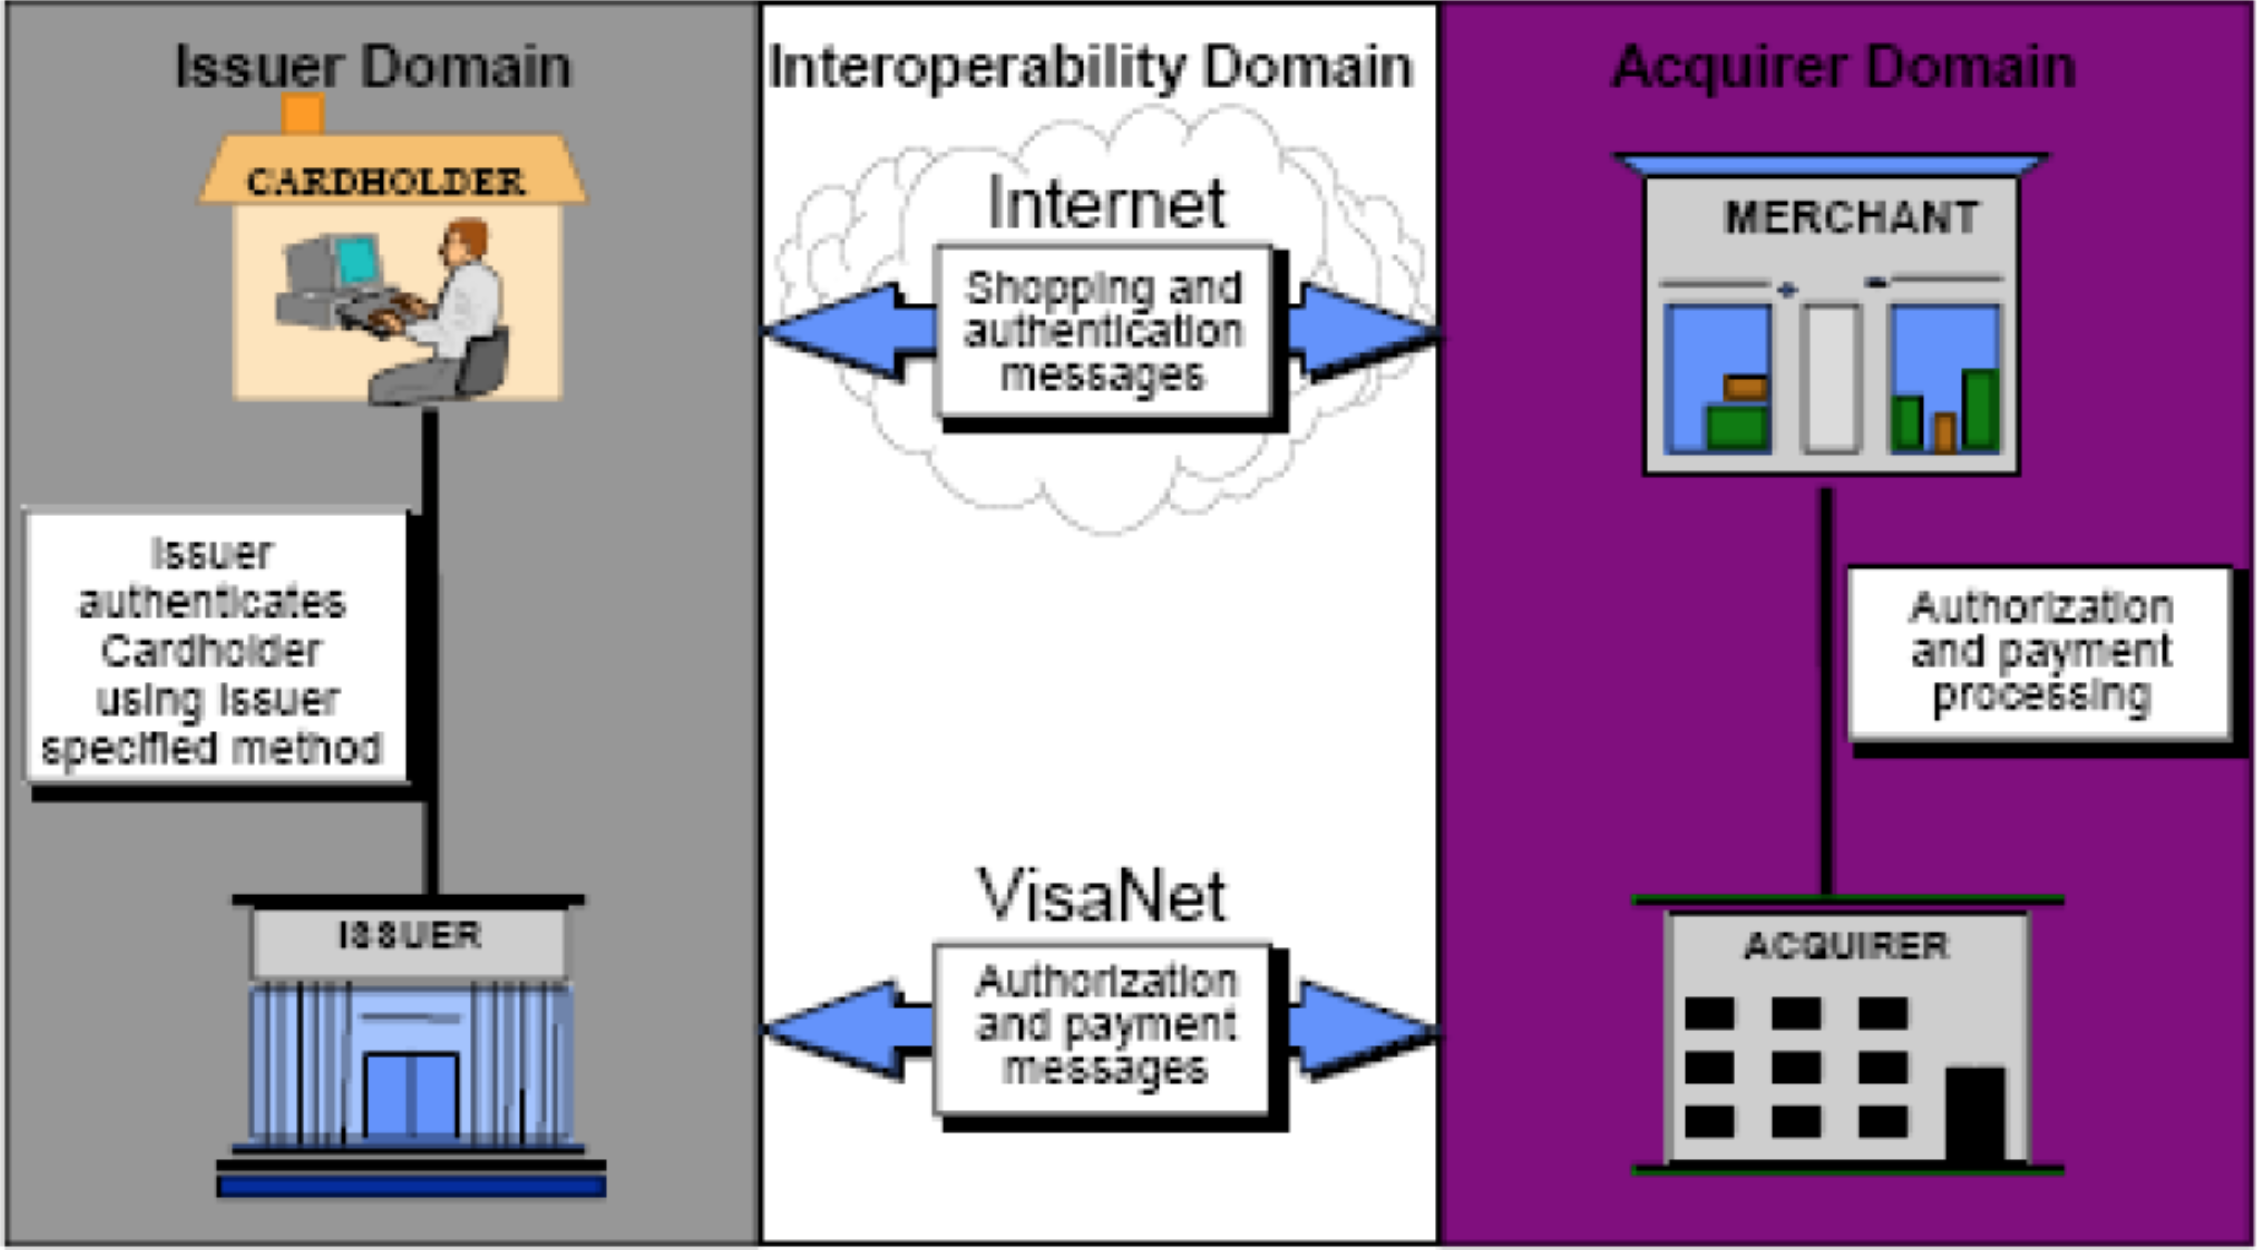
\includegraphics[width=\columnwidth]{img/3DSecure.png}
      After entering payment card details on merchant site:
      \begin{itemize}
        \item 3D Secure pops up a password entry form to a bank customer
        \item customer enters a password and, if it was correct,
        \item customer is returned to the merchant website to complete the
        transaction and
        \item the merchant gets an authorization code to submit to his bank
      \end{itemize}

      \textbf{Problems}: Pop-Up blockers (changed to iframes), Activation during shopping (phishing attacks), SLL verification not visible, liability shift (customer becomes liable for losses), weak bank authentication, no password reset procedure, privacy issues
    }

    \sectionbox{
    \subsubsection{802.1x : Port-Based Network Access Control}
      Client-server based access control protocol that restricts unauthorized devices from connecting to a (W)LAN through publicly accessible ports.

      For each 802.1x switch port, the switch creates \textbf{TWO virtual access points} at each port. The controlled port is open only when the device connected to that port has been authorized by 802.1x

      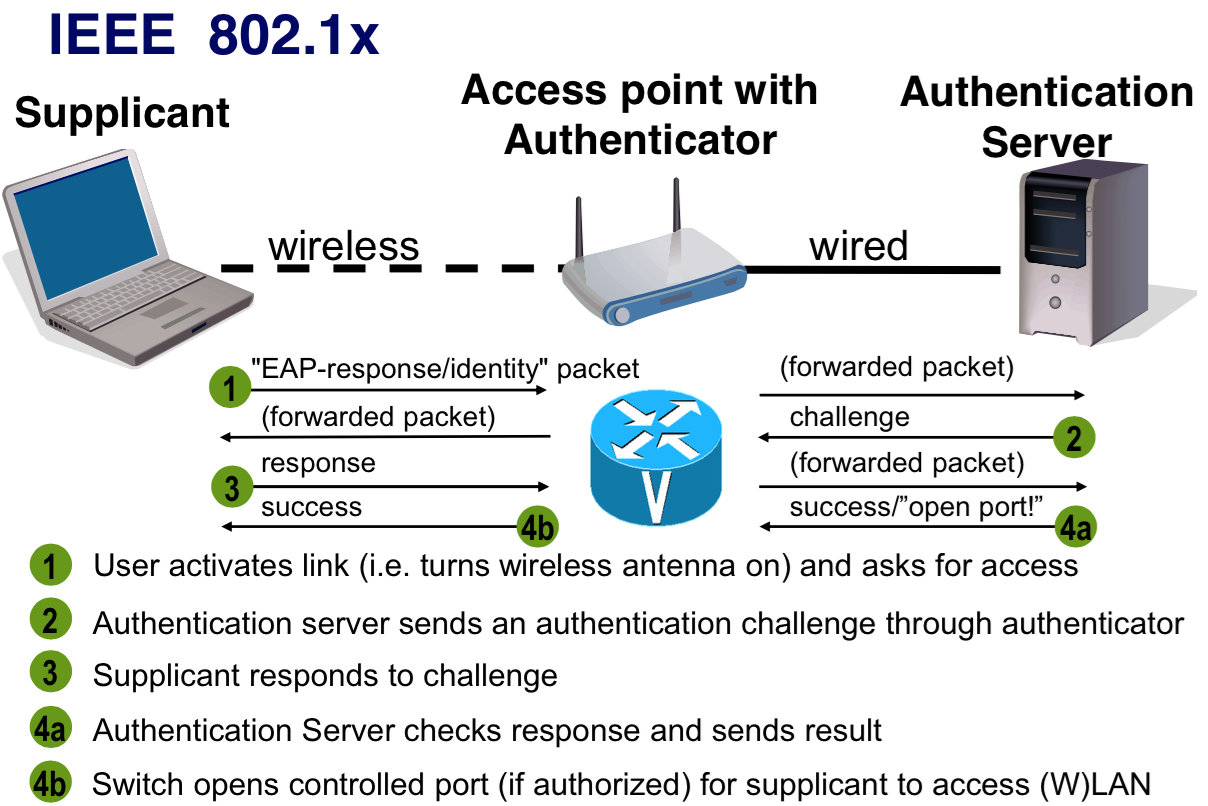
\includegraphics[width=\columnwidth]{img/8021x.png}

      \textbf{EAP} (Extensible Authentication Protocol): Authentication framework on the data link layer supporting multiple methods (MD5, OTP=one-time passwords, TLS, TTLS) without requiring an IP.

      \textbf{Roles : Identity and Security}: Authentication (Who?) , Authorization (What?) , Access Control, Policy enforcement

      \textbf{Benefits:} Standard based technology, control at link layer, interoperating wifi and wired, centralized user administration

      \textbf{Drawbacks:} Authenticator authentication, Man-in-the-middle, session hijacking
    }

    \sectionbox{
      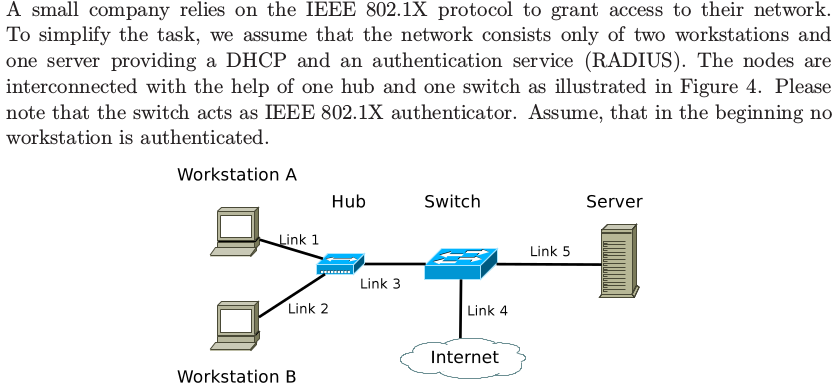
\includegraphics[width=\columnwidth]{img/8021x_exam.png}

      \begin{enumerate}
        \item Workstation A sends a DHCP request toward the DHCP server $\ra$ there is no reply, the request is blocked at the switch. Only EAP queries pass through the uncontrolled port are allowed by the switch.
        \item Workstation A sends an EAP-Response packet $\ra$ links 1,2,3,5 can see this packet.\\
        Now assume the Workstation A is authenticated using 802.1x.
        \item Workstation B tries to access http://www.example.com on the Internet $\ra$ He receives an answer because A opened the port on the switch for both machines.
        \item In this network, IEEE 802.1x does NOT prevents malicious users/hosts to steal HTTP session cookies. 802.1x does not provide any encryption and both users are connected with a cable.
        \item The IEEE 802.1x protocol does NOT require fully functional DHCP and DNS services since it operates on OSI layer 2 (link/MAC layer), nothing above this layer is required.
      \end{enumerate}
    }

    \sectionbox{
    \subsection{Anonymization}
      There is no perfect anonymity in reality.

      \textbf{Levels of Anonymity:} Identity (principal known), Pseudonymity (indirectly kown as pseudonym), anonymity (part of anonymity set but no distinguishing within)

      \textbf{Pseudonyms:} public (\ra identification), non-public (\ra pseudonymity), unlinkable (\ra anonymity)

      \textbf{Use cases:} \\
      \underline{physical}: feedback, voting, whistleblowing, censorship \\
      \underline{digital}: digital cash, digital voting, illegal activities

      \textbf{Oninon routing: } Data is encapsulated multiple times and only the next hop is known to each node (Default TOR = 3 nodes)

      \textbf{Mixnet:} proxy handles messages in batches (transformed and premutated) \Ra unlinkability of incoming and outgoing messagesat each proxy

      \textbf{Attacks:} Traceback (break systems on path - defense : more proxies), Collusion (bad nodes - defense : reputation system), Traffic analysis (tagging with bit errors, replay messages - defense: heartbeats, traffic shaping, padding messages to constant size) , Logging (most initiators want to continue end-to-end communication across path changes, compromised proxy records predecessor;Required server relays:TOR first and last, Mixnet all)
    }


\section{Firewalls, IDS and NAT Traversal}
    \sectionbox {
    \subsection{Firewall Attack techniques}
      \begin{itemize}
        \item IP source spoofing (doesn't work well with TCP based attacks)
        \item Artificial Fragmentation
        \item Vulnerabilities
        \item Denial of Service (state explosion)
        \item Tunnelling/Covert channel (ICMP, DNS\ldots)
      \end{itemize}
  }

  \sectionbox {
  \subsection{Firewall detection}
    \begin{itemize}
      \item \textbf{Port scanning}: traceroute, source IP of response $\ra$ improve obscurity by spoofing src address as target host
      \item \textbf{TTL}: let expire TTL one hop past firewall $\ra$ reset low TTL, spoof or create response
      \item Trying to keep existence of firewall secret is OK, but it's \textbf{not a security technique}
    \end{itemize}
  }

  \sectionbox {
  \subsection{Oranizational challenges}
    \begin{itemize}
      \item \textbf{Large Rulesets}: complex, hard to manage and understand
      \item \textbf{Big Organizations}: tools for hundreds of FW, process to change?
      \item \textbf{Conflict}: Networking vs. security staff
    \end{itemize}
  }

  \sectionbox{
  \subsection{Firewalls}
    Hardware or software device which is configured to permit, deny or proxy data through a computer network with different levels of trust. The configuration is called \emph{policy}.

    \textbf{Types:} simple packet filter, stateful filter, application layer proxy

    \textbf{Rules:} Filtering (outgoing (egress), incoming (ingress)), Default policy (accept, reject), Deny (Drop silently, Reject), Addressing Transparency (firewall and network fingerprinting)

    \subsubsection{Stateless Firewall}
      Examine on network layer, decision based on header

      \underline{Pro}: application independent, good performance and scalability

      \underline{Cons}: no state or application context, can't prevent probing

    \subsubsection{Stateful Firewall}
      Keeps track of state. Decision based on \emph{session state}

      \underline{Pro}: more powerful rules

      \underline{Cons}: no state for UDP, host vs. firewall state (inconsistent), state explosion

    \subsubsection{Application Layer Firewall}
      Take application state into account

      \underline{Pro}: application aware

      \underline{Cons}: many application protocols, performance, scalability

    \subsubsection{Web Application Firewall}
      Protects web-based applications from malicious requests (often reverse proxy)

      \underline{Filtering}: signatures, black/whitelisting
    }

  \sectionbox {
  \subsection{NAT (Network Address Translation)}
    One-to-one IP Address rewriting, keeps port numbers.

    \textbf{NAPT} = Network Address and Port Translation (Most used one) is  many-to-one (multiple hosts on private network using the same public IP address)

    \textbf{Benefits}: Saves address space + Prevents malicious activity from outside (Don't use it for security as a Firewall)

    \textbf{Drawbacks}: no end-to-end connectivity + P2P and IPSec don't work

    \subsubsection{NAT UDP Hole Punching (using RDV server)}

    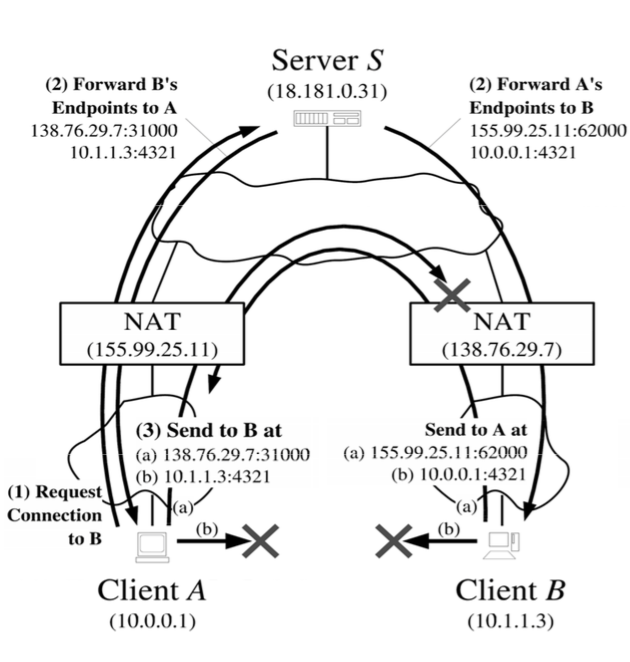
\includegraphics[width=\columnwidth]{img/nathole.png}

    \subsubsection{NAT Security}
    No protection against application vulnerabilities once a connection is established. Prevents outsiders to initiate a connection. Network discovery through NAT is possible. NATs allowing hole punching for P2P may be vulnerable
  }

  \sectionbox {
  \subsection{Firewall configuration : IP Tables}
    Rule (source destination port/IP and target):
    \texttt{iptables -A INPUT -p tcp -s 0/0 -d 0/0 --dport 80 --syn -j ACCEPT}

    \textbf{Rule Targets}(when packet matches rule)

    ACCEPT; DROP; REJECT; QUEUE–(rarely used); RETURN–(rarely used);

    MASQUERADE–only in nat table: rewrite source or destination address with address of outgoing or incoming interface
  }

  \sectionbox{
  \subsection{Intrustion Detection and Prevention Systems}
    Try to detect intrusions on the network by comparing to attack signatures. Block traffic after detection. \textbf{Output:} alerts, action, reporting, analysis

    \subsubsection{Classification}
      \textbf{Object of observation:}

      \underline{Packet}: (-)IP fragmentation, (-)not scalable (explosion)

      \underline{Flow}: (+)scalability, (+)encryption not problem, (-)not content-based

      \textbf{Point of observation:}

      \underline{Host}: (-)hard deployment, (+)context information, (+)one sensor per machine

      \underline{Network}: (+)easy deployment, (+)multiple machines, (-)unknown machines, (-)performance (no context)

      \textbf{Method of observation:}

      \underline{Signature}: (+)precision, (-)not detecting unknown attacks

      \underline{Behavior}: (+)unknown attacks, (-)difficult to find ground truth, (-)false positives

    \subsubsection{Challenges}
      \begin{itemize}
        \item False alarms and false silences
        \item Cope with high network speeds
        \item Sensor management and signature distribution
        \item Policy management
        \item Manpower for interventions 24x7
      \end{itemize}

    \subsubsection{Attacks and IDS evasion techniques}
    DoS attacks can also be used as a component of an attack. It enables other attacks to remain undetected.
      \begin{itemize}
        \item Flooding / resource exhaustion
        \item algorithmic Complexity Attacks (e.g. on hash table) $\ra$ use some randomness
      \end{itemize}
  }


\section{The Domain Name System Security}

  \sectionbox{
  \subsection{Routing}
    \textbf{ASes}(Autonomous System): define by AS Number $\simeq 40000$
    \begin{itemize}
      \item \underline{Tier 1ISP}: can access all internet for free or by reciprocal agreement
      \item \underline{Transit}: AS transiting msg for other (for \$)
      \item \underline{Tier 2ISP}: need to purchase transit
    \end{itemize}

    \subsubsection{BGP (Border Gateway Protocol)}
      Used to exchange routing and exchangeability information (inter ASes $\ra$ \textbf{iBGP}, between ASes $\ra$ \textbf{eBGP})

      BGP routers have Routing Information Base (RIB) $\ra$ if update its RIB $\Ra$ notify others around

      \textbf{Attacks on BGP}: eavesdropping, replay, msg insertion, deletion and modification, MitM, DOS + TCP attacks (reset attack)

      \textbf{Solutions}: BGP + TCP MD5 signature (not efficient), SBGP, SCION
  }

  \sectionbox{
  \subsection{Attacks on DNS}
    \subsubsection{Denial of Service on DNS}
      Targeting the 13 DNS root servers which are a bottleneck resource.

      \textbf{Defense}: Over-provisioning (13 clusters) + Anycast (\textgreater 500) (1 address to multiple potential receivers) prevents most attacks.

    \subsubsection{Account-Takeover}
      Attacking the web interfaces of registrars and try to enter malicious name servers. Possible solution: Multi-channel authentication

    \subsubsection{Manipulate local DNS settings}
      \begin{itemize}
        \item Manipulate local host configurations (access to the local machine nescessary)
        \item Spoof DHCP replies (access to LAN nescessary) \ra countermeasure: authentication for DHCP messages
        \item Set up Malicious DHCP server that is faster than the valid one
      \end{itemize}

      \textbf{Example:} DNS-Changer-Botnet (4million infected hosts, difficult malicious DNS servers shut-down : still used by at least 250 000 hosts)

    \subsubsection{DNS Spoofing}
      Successful insertion of incorrect resolution information by a host that has no authority to provide that information. Attacker sniffs traffic for a victim request and get the TXID. He can reply with the right TXID. Works only if attacker is faster than legitimate DNS Response.

    \subsubsection{Manipulate DNS lookup process (Cache Poisoning)}
      Inject faked Domain,IP information into caching name server.

      \underline{Process}: attacker asks caching server for attack.com, attacker server replies with fake records in the additional section (e.g. www.bank.com)

      This worked because early DNS implementations accepted records in the additional section without proper checking.

      \textbf{Bailiwick Checking}: Is the server authorized to respond to DNS requests for the domain. They check the hierarchy : 83.www.bank.com can return any record for www.bank.com but cannot for bank.com (which cannot for .com)

      \textbf{Weak authentication:} Port, TXID, Query string - first good answer wins

    \subsubsection{The Kaminsky Attack}
      \begin{enumerate}
        \item Inject query on the client \textit{\$Random}.www.bank.com
        \item reply multiple times  (TXID 0-200)
        \item Send name server redirections in additional section
        \item if it fails, return to step 1
      \end{enumerate}
      $\Ra$ Fix: Source Port Randomization. Chance: $65536 \cdot (65536 - 1024)$ to 1
  }

  \sectionbox{
  \subsection{DNS}
    \emphbox{DNS is a global, distributed, robust system for name to IP address resolution}

    DNS is the glue of the internet: Nearly all activities start with a DNS lookup (Orginally: no security considerations)

    Design:
    \begin{itemize}
    \item Client-Server application
    \item Hierarchical System
    \item Use UDP on port 53
    \end{itemize}

    \textbf{Zone:} Collection of hostnames/IP pairs managed together by same entity

    \textbf{Domain:} just a name, part of hierarchy of the DNS

    \textbf{Nameserver (authoritative): } Server that answers DNS queries (Responsible DNS Server for each zone)

    \textbf{Resolver:} Client part of DNS that resolves domain names

    \textbf{Recursive name server:}  Answers queries for all zones (1- Root Server, 2- TLD Server, 3- Authoritative DNS Server)

    \textbf{Stub resolver:} Forwards request to recursive name server (typically used by end-hosts)

    \textbf{Caching:} Reduces overhead. Lifetime controlled by TTL

    \texttt{dig URL\_TO\_LOOKUP @DNS\_SERVER} = make a request to a specific DNS

    \texttt{whois IP\_OR\_URL\_TO\_LOOKUP} = get information on a specific IP or URL

    \texttt{nslookup URL\_TO\_LOOKUP} = get IP address from a URL (don't use OS local DNS as \texttt{dig})

    3 possible answers to DNS queries:
    \begin{itemize}
      \item Here is your answer
      \item go away
      \item I don't know ask \ldots
    \end{itemize}
  }

  \sectionbox{
  \subsection{DNSSEC}
    \underline{Provides}: Authenticity, Integrity, Backward compatibility

    \underline{Drawbacks}: No confidentiality, No protection against DoS, Must be installed from a trusted source, Must be deployed at each step in the domain lookup.

    All records are signed: Key pairs for each zone $\ra$ Integrity

   Chain of trust $\ra$ Authenticity

   \textbf{DNS record types specific to DNSSEC}
   \begin{itemize}
     \item \textbf{ZSK}: Zone-Signing Keys (RRset signed with ZSK\_priv $\ra$ RRSIG)
     \item \textbf{RRSet}: Resource Record Set of the same type records
     \item \textbf{RRSIG}: Contains a cryptographic signature of RRsets
     \item \textbf{DNSKEY}: Contains a public signing key (ZSK or KSK)
     \item \textbf{KSK}: Key-Signing Keys, signs DNSKEY records of public ZSK creating a RRSIG record
     \item \textbf{ZSK}: Zone-Signing Keys, each zone has a/several pair(s) used to sign all other records (priv: signs, pub: verifies)
     \item \textbf{DS}: Contains the hash of a DNSKEY record
   \end{itemize}

   \textbf{To validate .ch:}
  \begin{enumerate}
    \item Request the KSK key of .ch by querying the parent zone (here, root) for a DS record (record set signed in RRSIG by root's ZSK)
    \item Verify RRSIG of DS record with root's public KSK (must be stored localy)
    \item Request desired RRset to contact .ch (containing A and NS records for .ch), with the corresponding RRSIG to sign it (using the .ch's ZSK)
    \item Request DNSKEY of .ch with public ZSK(s) and KSK with the RRSIG of DNSKEY RRset (using the domain's KSK)
    \item Verify RRSIG of RRset with the .ch's public ZSK
    \item Verify the .ch KSK key by hashing it and comparing it to the DS received in 1
  \end{enumerate}

   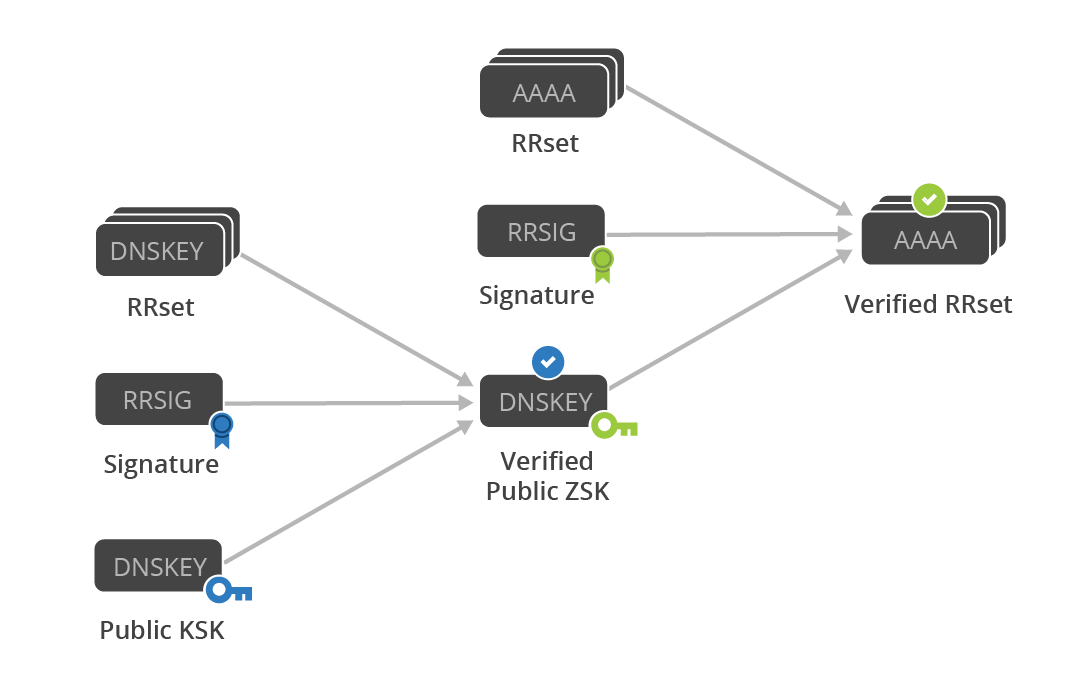
\includegraphics[width=\columnwidth]{img/DNSSECzone.png}

   There are two signing keys (ZSK and KSK) because the KSK is longer (i.e more secure and less often changed and used) than the ZSK (which can be changed more often and is used to sign a lot more records). The parent zone signs the KSK (not done often) which in turn can sign the ZSK (faster to use shorter keys).

   The DS (Delegation Signer) record glues the chain of trust :

   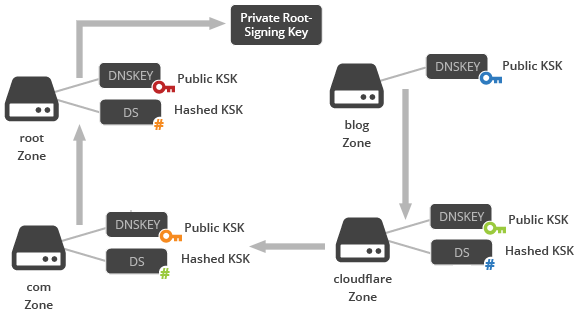
\includegraphics[width=\columnwidth]{img/DNSSECchain.png}
  }

\section{Availability and Denial of Service}
  \sectionbox{
  \subsection{System Level Agreements (SLA)}
    \begin{tabular}{ l | l | l | l }
      Level & \% & Downtime (year) & Downtime (month) \\ \hline
      Two-nines & 99 & 3.65 days & 7.2 hours\\
      Three-nines & 99.9 & 8.76 hours & 43.8 minutes \\
      Four-nines & 99.99 & 52.56 minutes & 4.38 minutes \\
      Five-nines & 99.999 & 5.26 minutes & 25.9 seconds \\
      Six-nines & 99.9999 & 31.5 seconds & 2.59 seconds \\
    \end{tabular}

    How to achieve 99.999:
    \begin{itemize}
      \item High Redundancy + Fast Failover (Quick Change)
      \item Failure Resilience
      \item Over Provisioning
      \item Backup, Close Monitoring and Fast Recovery
    \end{itemize}
  }

  \sectionbox{
    \subsection{Denial of service (DoS)}
      DoS attack : aims to prevent legitimate users from accessing a specific service. $\ra$ Resource starvation of CPU, Storage, Network

    \textbf{Attacks}:
    \begin{itemize}
      \item \underline{SYN-Flood}: Spam Server with TCP SYNs $\ra$ needs to keep state \emph{Solution}: Choose carefully constructed initial sequence number (crypto based) and SYN cookies (client keep state and present it later)
      \item \underline{Compression Bomb} \emph{Solution} :restrictions on size, depth and time
      \item \underline{Source Spoofing/Reflector Attack} from any vulnerable service, by botnet or broadcast addresses (Smurf attack)
      \item \underline{Mail Bounce}: reply-to: @victim.com, To: and multiple invalid Bcc: @target.com $\ra$ victim will receive many bounce emails from target.com
      \item \underline{DNS Amplification}: Send small request to recursive servers with spoofed source
    \end{itemize}
  }

  \sectionbox{
  \subsection{Dos Countermeasures}
    \textbf{Prevention}:
    \begin{itemize}
      \item \underline{Secure systems}: (e.g. prevent machine compromise to build botnets by patching, IDS/IPS, firewall etc.)
      \item \underline{Secure protocols}: (e.g. prevent IP spoofing, use TCP SYN
      cookies, HashCash: add client CPU cycles)
      \item \underline{Resource accounting}: (server commits resources only to
      authenticated/trustworthy clients)
      \item \underline{Resource multiplication}: (resource over provisioning for the case of an attack)
      \item \underline{Late resource binding}: (bind resources as late as possible)
    \end{itemize}

    \textbf{Reaction}:
    \begin{itemize}
      \item \underline{Detect} (using pattern, anomaly, third party)
      \item \underline{React} (rate-limit, filter, reconfigure, identify agents)
    \end{itemize}
  }

  \sectionbox{
  \subsection{Data Sizes : SI Vs Binary symbols}
    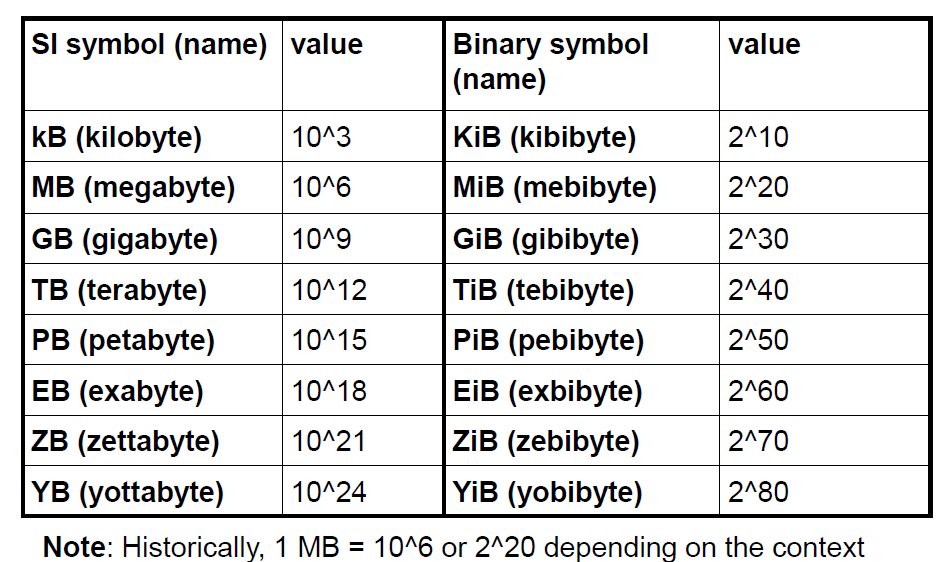
\includegraphics[width=\columnwidth]{img/sizesTable.PNG}
  }

\section{Secure Channels: Principles, VPN, SSH}

  \sectionbox{
  \subsection{Security by Layer of the TCP/IP Model}
    Properties of a secure channel: secure = authentic and confidential

    \subsubsection{Security at Link Layer}
      \begin{itemize}
      \item All traffic over a specific Link (WPA2 uses AES)
      \item Often implemented in hardware (Quantum Cryptography)
      \end{itemize}

      \underline{Pro}: Speed, Seamless

      \underline{Cons}: every link separately, trust in link operator

    \subsubsection{Security at Network Layer}
      Secure traffic over multiple links between end points (IPSec, L2TP)

      \underline{Pro}: seamless security to above layers, IPSec part of IPv6 + IPv4

      \underline{Cons}: complex configuration, tunnel mode encrypts only part of a route

    \subsubsection{Security at Transport Layer}
      Implemented in end-hosts (e.g. TLS/SSL, SSH)

      \underline{Pro}: can be added to existing apps, portable and easy configuration

      \underline{Cons} (of TLS): protocol specific(TCP), application must be TLS/SSL aware

    \subsubsection{Security at Application Layer}

      implemented in end hosts (PGP, S/MIME, Skype, \ldots)

      \underline{Pro}: extend app without involving OS, applications understand data

      \underline{Cons}: separate security for each app
  }

  \sectionbox{
  \subsection{SSH}
    Standard for remote login and encrypted file transfer, provide PFS.
    Security algorithms and parameters used are negotiable.

    \subsubsection{Protocols}
      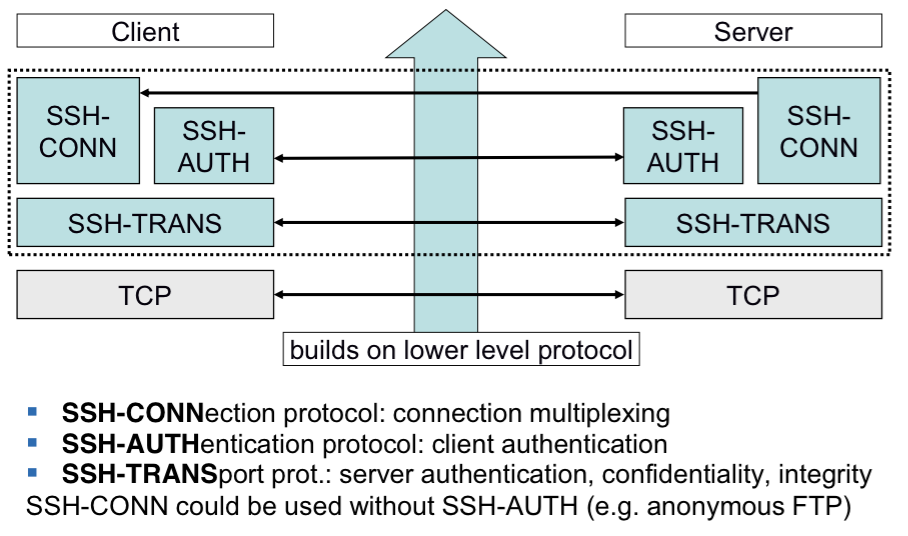
\includegraphics[width=\columnwidth]{img/sshproto.png}

    \subsubsection{SSH-Trans}
      \begin{itemize}
        \item algorithm negotiation
        \item session key exchange (e.g. Diffie-Hellman)
        \item session id
        \item server authentication
        \item encryption, integrity, data compression
      \end{itemize}

    \subsubsection{SSH-Auth}
      \begin{itemize}
        \item authenticates the client with multiple auth mechanisms
        \item defines format of auth-requests (Username, Method name, Service name)
      \end{itemize}

    \subsubsection{SSH-Conn}
      \begin{itemize}
        \item multiplexing multiple steams
        \item port forwarding
        \item compression handling
        \item interactive and non-interactive sessions
      \end{itemize}

    \subsubsection{Attacks SSH cannot counter}
      \begin{itemize}
        \item password cracking (passwords must be strong and not reused)
        \item traffic analysis
        \item IP and TCP attacks
      \end{itemize}
  }

  \sectionbox{
  \subsection{VPN}
    Securely interconnect networks or machines over an existing network.\\
    IPSec, L2TP, OpenSSH, SSL/TLS can tunnel entire network's traffic (OpenVPN).\\

    \begin{itemize}
      \item Encryption $\ra$ confidentiality
      \item Randomized Initialisation Vectors (IVs)
      \item Replay protection $\ra$ unique ID or timestamp in packets before signature
      \item Authentication (HMAC) $\ra$ integrity and authenticity
    \end{itemize}

    \subsubsection{Tunnel Mode (Gateway-to-Gateway)}
      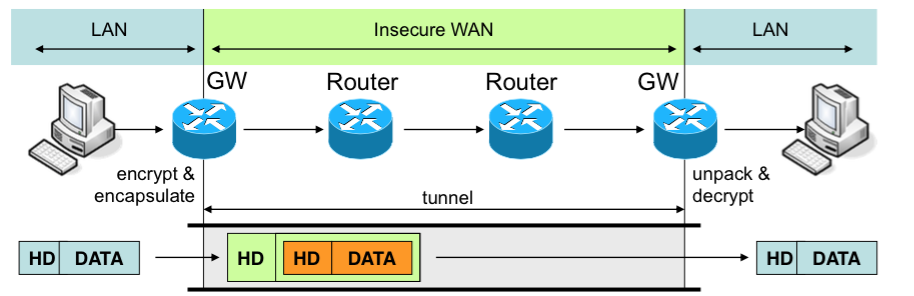
\includegraphics[width=\columnwidth]{img/vpntunnel.png}
      \begin{itemize}
        \item Encrypt and Authenticate original IP packet
        \item Transport it as payload in new IP packet (IP encapsulation)
        \item \textbf{IPSec Tunnel Mode} packet architecture :
      \end{itemize}
      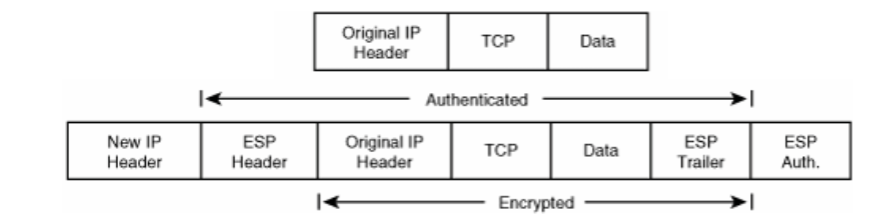
\includegraphics[width=\columnwidth]{img/vpntunnel2.png}

    \subsubsection{Transport Mode (End-to-End)}
      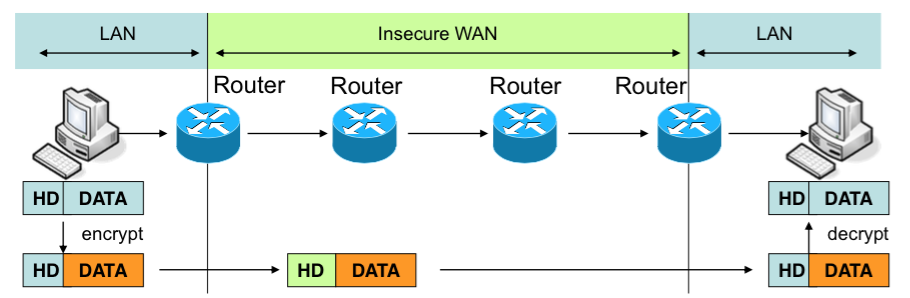
\includegraphics[width=\columnwidth]{img/vpntransport.png}

      \begin{itemize}
        \item End-to-End communication between hosts
        \item Encrypt and Authenticate payload only
        \item \textbf{IPSec Transport Mode} packet architecture :
      \end{itemize}

      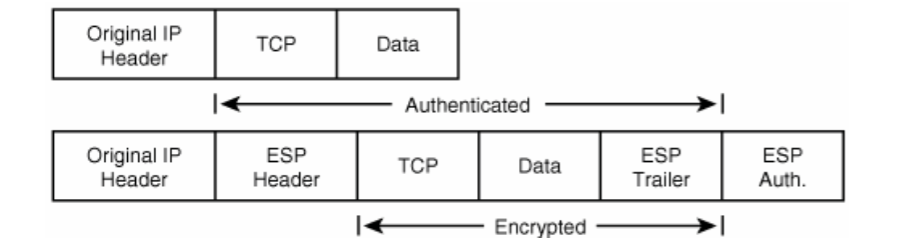
\includegraphics[width=\columnwidth]{img/vpntransport2.png}

    \subsubsection{IPSec Security Association (SA)}
      A Security Association (SA) is the establishment of shared security attributes between two network entities to support secure communication.

      SA is uniquely defined by a triple of :
      \begin{itemize}
        \item Security Parameter Index (SPI): number placed in ESP datagrams.
        \item IP Destination Address
        \item Security Protocol Identifier:AH or ESP
      \end{itemize}
  }

  \sectionbox{
  \subsection{Message Authentication Code (MAC)}
    Provide data integrity and authentification
    \begin{itemize}
      \item message not modified in transit
      \item source is authentic
      \item not delayed
      \item sequence order
    \end{itemize}

    \texttt{MAC (K, M) = DES (K, M)} take last 32 bits

    \subsubsection*{HMAC (Mac with Hash functions)}
    \begin{itemize}
      \item use hash functions (MD5, SHA)
      \item faster
      \item easy available
      \item less affected by collisions than hash functions $\ra$ if MD5 or SHA-1 broken, corresponding HMAC can still be secure.
    \end{itemize}

    \texttt{HMAC (K, M) = H(K' xor opad | H (K' xor ipad | M))}
  }

\section{TLS (Transport Layer Security)}
  \sectionbox{
    \begin{itemize}
      \item Session or Application layer (OSI model)
      \item SSL (Secure Socket Layer) = predecessor of TLS
      \item SSLv3 and TLS almost same except some crypto algo.
    \end{itemize}
  }

\sectionbox{
\subsection{Diffie-Hellman Key Exchange (DH)}
  \begin{itemize}
    \item \textbf{Public	values}:	large	prime	$p$,	generator	$g$
    \item \textbf{Secret values}: Alice	has	$a$,	Bob	has $b$
    \item Alice	$\ra$ Bob:	$A = g^a \pmod{p}$
    \item Bob	$\ra$ Alice:	$B = g^b \pmod{p}$
    \item Bob computes	$A^b	\pmod{p}=	g^{ab}\pmod{p}$
    \item Alice	computes $(B)^a	\pmod{p}=	g^{ab}\pmod{p}$
    \item Alice and Bob have now a shared secret $g^{ab}\pmod{p}$
    \item Eve	cannot	compute	$g^{ab}	\pmod{p}$
  \end{itemize}
}

\sectionbox{
\subsection{Generation of Crypto Parameters}
  \textbf{Master Secret}(MS) created from pre-master secret(PS), client random(CR), server random(SR): MS = $h('A') || h('BB') || h('CCC')$

  with $h(X) = MD5(PS || SHA(X || PS || CR || SR ))$

  \textbf{Key materials} pairs client \& server: MAC key, write key and write IV \texttt{key\_block} = $h_2('A') || h_2('BB') || h_2('CCC') || \cdots$

  with $h_2(X) = MD5(MS || SHA(X || MS || CR || SR ))$
  \begin{itemize}
    \item \texttt{key\_block} is the concatenation of the 6 keys
    \item Nb of round depends on size of keys $\ra$ MD5 = 16 bytes per round
    \item MS $\simeq$ pseudorandom seed value and CR and SR $\simeq$ salt values
  \end{itemize}
}

  \sectionbox{
  \subsection{Key Exchange Methods}
  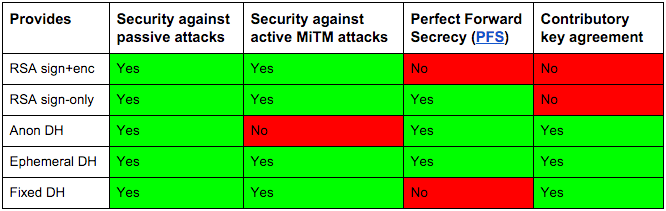
\includegraphics[width=\columnwidth]{img/Key-Exchange-Algorithms.png}

  \begin{itemize}
    \item \textbf{Contributory Key Agreement} = Both parties contribute to session key, no party can fully determine session key.
    \item \textbf{Perfect Forward Secrecy} = knowing long-term private key does not reveal session key.
  \end{itemize}

  \subsubsection{RSA}
    Pre-master secret(PMS)= 48-bytes (2 protocol version + 46 random)\\
    \textbf{sign+enc}: client generates pre-master and encrypts it with $PU_{server}$.
    \begin{itemize}
      \item No \texttt{server\_key\_exchange} msg needed in phase 2
      \item Always same public/private keys used $\Ra$ no PFS $\Ra$ Not recommended
    \end{itemize}

    \textbf{sign-only}: Server RSA keys used for signature only
    \begin{itemize}
      \item Server creates temporary RSA keys, signs them with $PR_{server}$ and use \texttt{server\_key\_exchange} to send them
      \item PMS encrypted with temporary server public key
    \end{itemize}

  \subsubsection{Diffie-Hellman}
    \textbf{Anonymous DH}: No authentication of client nor server
    \begin{itemize}
      \item \texttt{server\_key\_exchange}: DH public values + server public DH key
      \item \texttt{client\_key\_exchange}: client public DH key
      \item Vulnerable to MitM attacks
    \end{itemize}

    \textbf{Ephemeral DH}: create ephemeral (one-time) secret keys
    \begin{itemize}
      \item \texttt{server\_key\_exchange}: DH public values + server public DH key + signature of those parameters
      \item \texttt{client\_key\_exchange}: client public DH key
      \item Don't provide authentication but signing values with RSA does.
      \item Most commonly used
    \end{itemize}

    \textbf{Fixed DH} : DH public values + server public values are fixed
    \begin{itemize}
      \item All DH parameters in server certificate signed by CA $\Ra$ no need of \texttt{server\_key\_exchange}
      \item server can asked client to be authenticated with \texttt{certificate\_request}
      \item Rarely used
    \end{itemize}
  }

  \sectionbox{
  \subsection{Attacks against SSL/TLS}
    \subsubsection{Dumbing Down}
      \begin{itemize}
        \item attacker forces to use old breakable algo. for communication (using the \texttt{ciphersuite})
        \item only DOS except with anon DH where it can become real MitM
      \end{itemize}

    \subsubsection{Attacks against CAs}
      \begin{itemize}
        \item Attacks against CA to get false certificates signed
        \item any CA can issue certs for any domain (weakest link)
        \item 2010: Stuxnet signed itself 2 compromised Taiwan CAs' private keys
        \item 2011: Comodo was duped into creating certificates for Google sites
      \end{itemize}

    \subsubsection{BEAST}
      \begin{itemize}
        \item Vulnerability in the Initialization Vector (IV) of the CBC mode of AES
        \item  MitM can read msg by encrypting it multiple times
        \item mitigated in TLS1.1 and above
      \end{itemize}

    \subsubsection{Assumption for Secure TLS}
      \begin{itemize}
        \item CA, Crypto, Browser, User
        \item if a single assumption does not hold $\Ra$ TLS not secure
      \end{itemize}
  }

  \sectionbox{
  \subsection{Handshake Protocol}
    \subsubsection{Phase 1: Establish Security Capabilities (hello\_messages)}
      \begin{enumerate}
        \item C $\ra$ S: \texttt{client\_hello}
        \begin{itemize}
          \item \textbf{version}: highest supported version.
          \item \textbf{ciphersuite}: Supported ciphers listed in $\searrow$ order of pref.\\
          := Key exchange algo. + Cipher algo. (RC4, AES, 3DES…) + MAC algo. (MD5 or SHA-1) + \dots
          \item \textbf{random}: 32-bit timestamp + 28 bytes random $\Ra$ prevent replay
          \item \textbf{compression}: list of compression methods
          \item \textbf{SessionID}: update (value=which session) or create (value=0)
        \end{itemize}
        \item S $\ra$ C: \texttt{server\_hello}: Reply to every param.
      \end{enumerate}

    \subsubsection{Phase 2: Server Authentication and Key Exchange}
      \begin{enumerate}
        \item S $\ra$ C: \texttt{certificate}*: except for Anon DH, contains public DH param if DH fixed used
        \item S $\ra$ C: \texttt{server\_key\_exchange}*: required for Anon DH, Ephemeral DH, RSA sign-only
        \item S $\ra$ C: \texttt{certificate\_request}*: request types of cert. from client
        \item S $\ra$ C: \texttt{server\_hello\_done}: no param. + wait for client response
      \end{enumerate}

    \subsubsection{Phase 3: Client Authentication and Key Exchange}
      Client should verify server certificate (if required) + server parameters
      \begin{enumerate}
          \item C $\ra$ S: \texttt{certificate}*: client cert. or \texttt{no\_certificate} alert
          \item C $\ra$ S: \texttt{client\_key\_exchange}
          \begin{itemize}
            \item \textbf{RSA}: 48 bytes pre-master secret encrypted with server’s public key
            \item \textbf{DH}: client public DH values
          \end{itemize}
          \item C $\ra$ S: \texttt{certificate\_verify}*: hash of master secret + previous msgs encrypted with client private key (except fixed DH)
      \end{enumerate}

    \subsubsection{Phase 4: Finish}
    \begin{enumerate}
      \item C $\ra$ S: \texttt{change\_cipher\_spec}: Send 1 byte to confirm encryption.
      \item C $\ra$ S: \texttt{finished}: hash( master\_secret $||$ pad2 $||$ hash( handshake\_messages $||$ Sender $||$ master\_secret $||$ pad1 ))
      \begin{itemize}
        \item once with MD5(...) and once with SAH-1(...)
        \item \texttt{handshake\_messages} = all messages until now
      \end{itemize}
      \item S $\ra$ C: \texttt{change\_cipher\_spec}: server confirm encryption too
      \item S $\ra$ C: \texttt{finished} 1st encrypted msg = hash of all previous msg
    \end{enumerate}

  \textit{* = optional or situation-dependent messages that are not always sent}
  }

  \section{Certificates and PKI (Public Key Infrastructure)}

    \sectionbox{
    \subsection{Public-Key Certificates}
      Certificate = (public key + id of key owner)*signed by a trusted 3rd party
      \begin{enumerate}
        \item All can determine name + public key of the certificate’s owner
        \item All can verify signature of CA
        \item Only CA can create and update certificates
        \item All can verify the currency of the certificate
      \end{enumerate}

      \subsubsection{Revocation of Certificates}
      \begin{enumerate}
        \item User’s private key is assumed to be compromised
        \item User is no longer certified by this CA
        \item CA’s certificate is assumed to be compromised.
      \end{enumerate}
      \textbf{CRL}(Certificates Revocation List): listing of all the revocated certificates by a CA.
    }

    \sectionbox{
    \subsection{OCSP (Online Certificate Status Protocol)}
    Verify certificate status, ensure it is valid and has not been revoked.
      \begin{itemize}
        \item Small bandwidth needs $\Ra$ Real-time checks but not always reliable
        \item Privacy issues $\leftarrow$ OCSP responder can track users
        \item OCSP servers need to answer every client request (no cache)
        \item if connection fails, client has to make the choice on its own
        \item OCSP stapling: certificate owner give OCSP response with its certificate $\Ra$ \textbf{Not secure} active attacker dropping requests, default behavior is to validate for no responder
      \end{itemize}
    }

    \sectionbox{
    \subsection{GL: Certificate Transparency}
      Protocol for publicly logging the certificates activity.\\
      $\Ra$ augment chain-of-trust for the entire SSL certificate system.
      \begin{itemize}
        \item \textbf{Logs}: log cryptographically secured in a Merkle hash tree
        \item \textbf{Monitors}: watch for suspicious or missing certificates in logs
        \item \textbf{Auditors} : verify the overall integrity of logs (Signed Certificate Timestamp (SCT))
      \end{itemize}

      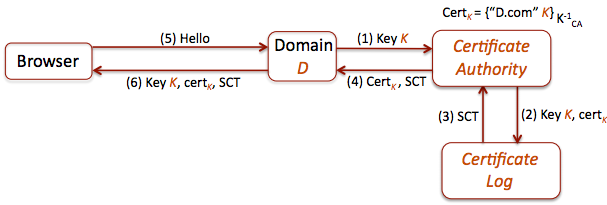
\includegraphics[width=\columnwidth]{img/CT.png}

      \textbf{Benefits:} Gradual rollout + Minimal impact on existing infrastructure

      \textbf{Disadvantages:} MitM (but can be detected externally), no support revocation, still need to contact log to verify
    }

    \sectionbox{
    \subsection{AKI (Accountable Key Infrastructure)}
      \begin{itemize}
        \item New public-key validation infra. to reduce lvl of trust in CAs
        \item Distribute trust $\ra$ no single point of failure
        \item support revocation and update of certificates
        \item Based on integrity tree (Efficient representation of the current state of all domains)
      \end{itemize}
    }

\section{Web Application Security}
  \sectionbox{
  \subsection{Top 10 Application Security Flaws}
    \begin{tabular}{ l | l }
      A1 & Injection (SQLi, LDAP, XPATH, OS Command)\\
      \hline
      A2 & Broken Authentication and Session Management\\
      \hline
      A3 & Cross-Site Scripting (XSS)\\
      \hline
      A4 & Insecure Direct Object References\\
      \hline
      A5 & Security Misconfiguration\\
      \hline
      A6 & Sensitive Data Exposure\\
      \hline
      A7 & Missing Function Level Access Control\\
      \hline
      A8 & Cross-Site Request Forgery (XSRF)\\
      \hline
      A9 & Using Components with Known Vulnerabilities\\
      \hline
      A10 & Unvalidated Redirects and Forward\\
    \end{tabular}\\
    \textit{OWASP (Open Web App Security Project), Nov. 2013}
  }

\section*{Session Management}
  \sectionbox {
  \subsection{Attacks}
    \begin{itemize}
      \item Network sniffing $\ra$ use HTTPS to prevent it
      \item Don't mix HTTP and HTTPS SessionID
      \item Random SessionID is important
      \item Brute Force $\ra$ Not predictable Username and Password
    \end{itemize}
  }

  \sectionbox {
  \subsection{Anatomy of a Web App \& Threat Vectors}
    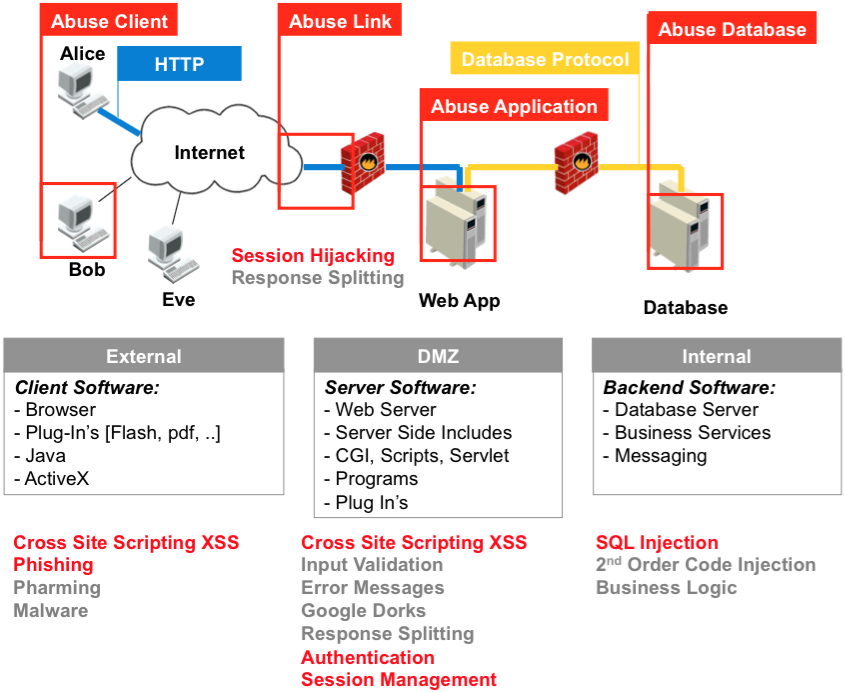
\includegraphics[width=\columnwidth]{img/webapp-threatvectors.png}
  }

  \sectionbox {
  \subsection{HTTP and Session Management}
    HTTP is stateless $\ra$ state needs to be implemented with session ID

    \textbf{SessionID}: generated on server, stored on client, transmitted with every request

    After login $\ra$ Identification by SessionID (Target for attacker)

  \subsubsection{Generation}
  \begin{itemize}
    \item Strong $\ra$ not predictive + impossible to guess next value
    \item Random $\ra$ not based on predictable values (no MD5 or SHA-1)
  \end{itemize}

  \subsubsection{Transport}
    \begin{itemize}
      \item GET: easy (in URL), (+)compatible , (-)logged on intermediate devices, (-)HTTP referer
      \item POST: (+)compatible(works with cookies disabled), (+)not obvious, (-)more complex development, (-)slightly harder to manipulate\\
      $\ra$ Both GET and POST are vulnerable to \emph{session fixation} attacks !
      \item Cookie: (+)more options, (+)not recorded, (+)https restriction, (-)store on client, (-)may be disabled by users
    \end{itemize}

  \subsubsection{Revocation}
  \begin{itemize}
    \item Session Validity: client and server side revocation + time limited
    \item Session Timeout: important with shared computers, expiry time should be minimum
  \end{itemize}

  \subsubsection{Destruction}
  % Important to keep because it is part of the all
  }

\section*{SQL Injection (SQLi)}
  \sectionbox{
  \subsection{Code Injection}
    Attack which insert code that is afterwards interpreted by a process.

    \textbf{Process:}
    \begin{enumerate}
      \item Data enters app from untrusted source
      \item Data is part of a string executed as a command by app
      \item App gives attacker privilege or info that he would otherwise not have
    \end{enumerate}
  }

  \sectionbox{
  \subsection{SQL Injection Defense}
    \begin{itemize}
    \item constrain and sanitize all client data on the server (input validation)
    \item use parametrized prepared statements
    \item use stored procedures (restraint possible actions)
    \item avoid disclosing error information
    \item run DB with reduced privileges
    \end{itemize}
  }

  \sectionbox{
  \subsection{SQL code injection}
    SQLi = insertion of SQL query via input data from client to app.

    \textbf{What can you do with it ?}
    \begin{itemize}
      \item Read / Modify data in the database
      \item Execute admin operations on the DB
      \item issue commands on the OS
    \end{itemize}

    \subsubsection{Tautology}
      Inject code in conditional statement(s) $\Ra$ always evaluate to true\\
      \texttt{SELECT uid FROM users WHERE login='\textcolor{red}{' OR ''='}' AND pwd='\textcolor{red}{' OR ''='}';}

    \subsubsection{Union Query}
      Inject \texttt{UNION} query $\Ra$ get union of the 2 queries. Need same number(\#columns, add same on in case) and type of parameters from both selected queries.\\
      \texttt{SELECT uid FROM users WHERE login=’\textcolor{red}{’ UNION SELECT cardNo from CreditCards WHERE uid=123; --} AND pass=’’;}

    \subsubsection{Piggy-Backed Queries}
      Inject query at the end of another query ($\Leftarrow$ Misconfiguration)\\
      \texttt{SELECT * FROM users WHERE uid=’abc’ AND password=’\textcolor{red}{’; DROP TABLE users; --}';}

    \subsubsection{Stored Procedure}
      Execute stored procedures present in the database\\
      \texttt{SELECT * FROM users WHERE uid=’abc’ AND password=’\textcolor{red}{’; SHUTDOWN; --}';}

    \subsubsection{Inference / Determine DB Engine}
      If DB doesn't return error msg $\Ra$ change behaviour of DB to guess (Blind Injection or Time Injection (e.g. example)\\
      \url{http://www.example.com/product.php?product_id=}\texttt{\textcolor{red}{100 AND IF(version() like ‘5\%’, sleep(15), ‘false’));--}}\\
      $\ra$ check MySQL version 5.x or not $\Ra$ if yes server delays answer 15s


    \subsubsection{Alternate Encodings}
    Fool scanning and detecting techniques with alternate encoding.\\
    \texttt{SELECT * FROM users WHERE uid=’abc’ AND password=’\textcolor{red}{’; exec(char(Ox73687574646f776e)); --}'}

    \begin{itemize}
      \item \texttt{;} $\ra$ terminates a command
      \item \texttt{--} $\ra$ considers everything afterwards as a comment.
      \item Error messages can provide hints on which DB is used.
      \item \textbf{IDS Detection Evasion} by varying the command (e.g. through the insertion of whitespaces or comments UNION/**/SELECT)
    \end{itemize}
  }

\section*{Cross-Site Scripting (XSS)}
  \sectionbox{
    \subsection{Same-origin policy}
      A script can only access content and properties of a document loaded from the same origin ($\Leftrightarrow$ same protocol, same hostname, same port but ignoring URL path)

      \textbf{Interaction of different origins}
      \begin{itemize}
        \item Link (href)
        \item iframe: Shown inside the website but can't exit iframe
        \item POST: POSTing data to external source (php form \ldots)
        \item script included: Evaluated in context of the website ($\Ra$ Dangerous)
        \item Asynchronous Requests (AJAX): Different origin only possible if allowed by target domain (with Access-Control-Allow-Origin Header)
      \end{itemize}
  }

  \sectionbox{
  \subsection{Request Forgery (XSRF)}
    A form from one domain posts a request to a different domain through an authenticated session (= write-only attack) (E.g.: Reset password)

    \textbf{Countermeasures:} (CSRF) hidden security Token (unique and cannot be read by attacker), ask for (old) password, check HTTP referer headers (indicates the page making the request, not always set $\ra$ not really efficient), show CAPTCHA
  }

  \sectionbox{
  \subsection{Script inclusion (XSSI)}
    \emph{Never include a script you do not trust!}

    \textbf{Direct sourcing}: honest server includes untrusted code from an external source

    \textbf{Call-back}: attacker’s website includes code (e.g.: scripts to send money) from an honest server which do not verify that the user really intended to execute it.

    \textbf{Countermeasures:} security tokens derived from the cookie and a server challenge, use only HTTP POST for XSSI call-back, check HTTP referer
  }

  \sectionbox{
  \subsection{XSS Attacks}
    XSS flaws occur whenever a web app takes user supplied datas and sends it to another web browser without first \emph{validating} or \emph{encoding} the content ($\Ra$ allows injection of malicious code).

    \textbf{Target:} The user of the web app

    \textbf{Infection path:}
    \begin{itemize}
      \item \underline{Reflected(1:1,URL)}: email, chat, uploaded files, third party content \ldots
      \item \underline{Stored}: script in database from forum messages, comments, username \ldots
      \item \underline{DOM Based}: stays in browser (DOM)
    \end{itemize}

    \textbf{Dangerous content:} advertisements, user contributed content, widgets (counters, scripts \ldots)

    \textbf{Example}: Data Leakage = script reads session cookies and sends them to an evil server ($\ra$ Solution: HTTPOnly cookies $\ra$ browser prevents client side script to access it, not supported by all browsers)

    \textbf{XSS Shell} = XSS backdoor and zombie manager $\ra$ can interactively send requests and get responses from victim ($\simeq$ backdoor the page)

    \subsubsection{Countermeasures}
      \begin{itemize}
        \item Test your web app
        \item Input sanitization (check user submitted content) $\ra$ filter out meta-characters ($<$, $>$, \ldots)
        \item HTML output encoding (escaping) $\ra$ e.g. $<$ is replaced by \&lt;
      \end{itemize}
  }

% Malware
\section{Malware}

  \sectionbox{
  \subsection{Definitions}
    \textbf{Malicious software (Malware)} is software that is intentionally included or inserted in a computer system for a harmful purpose.

    \textbf{Trojan}: seemingly offers useful functionalities but contains hidden functionality which undermine system security

    \textbf{Worm}: Self-contained software that can replicate itself from computer to computer across network connections. Upon arrival, may be activated to perform unwanted operation and continue propagating.

    \textbf{Bot}: malicious software agent running on a compromised machine executing commands by the bot master by listening to the command and control center (\textbf{botnet}= all bots listening to the same C\&C)

    \textbf{Rootkit}: activate during boot, hides from OS, can interfere with reflashing process or reinstall itself (self-healing)

    \textbf{Keylogger}: records keys pressed to steal information

    \textbf{Ransomware}: encrypt data and extort money for decryption key
  }

  \sectionbox{
  \subsection{Malware on Portable Storage}
    \begin{itemize}
      \item Uses Sneakernet(people) as physical propagation
      \item Variants: boot code virus (replaces boot sector), host program infection (embedding into executables)
      \item E.g. Stuxnet infected nuclear plants in Iran from USB sticks
    \end{itemize}
  }

  \sectionbox{
  \subsection{Problems cause by Malwares}

  \begin{itemize}
    \item Unauthorized use of system/network resources
    \item Sabotage
    \item Espionage
    \item Lowering of system security
  \end{itemize}
  }

  \sectionbox{
  \subsection{Malware detection}
    \textbf{Goal:} Detect malware and disinfect system

    \textbf{Deployment:} Endpoint, Network

    \textbf{Evaluation:} Recognition rate (high true positive), False alarm rate (low)

    \subsubsection{Signature Based}
      \begin{itemize}
        \item Reactive (based on known malware binaries)
        \item Signature database (keeps growing, polymorphism)
        \item Metrics: update delay, coverage, resource consumption
       \end{itemize}

    \subsubsection{Behaviour Based}
      \begin{itemize}
        \item Requires behavior model (ground truth, baseline)
        \item Problematic: user alerting (when is it a problem ?)
       \end{itemize}

     \subsubsection{Evaluation Antivirus Softwares}
        \begin{itemize}
          \item Detection (reactive, proactive)
          \item Support for compression
          \item Self-protection
          \item Cleanup of already infected system
          \item Enterprise deployment features
        \end{itemize}
  }

  \sectionbox{
  \subsection{Resistant Malware}
    \subsubsection{Antivirus Detection Evasion}
      \begin{itemize}
         \item Polymorphism (signature won't recognize them)
         \begin{itemize}
           \item different code with same effect (while instead of do - while)
           \item change order of code
           \item insert noise (sleep(0), if (1==1) or NOPs)
           \item compiler setting modulation (using different compiler options).
         \end{itemize}
         \item Code obfuscation (Disguise actual purpose)
         \item Encryption of code and messages
         \item Code changes to prevent disassembly
         \item Sandbox detection (act normal if monitored)
         \begin{itemize}
           \item read flags/API that would indicate the process is being debugged
           \item self debugging: failure indicates that the program is already being debugged
           \item measuring deltas between timestamps around exception handlers
         \end{itemize}
         \item Bootstrapping / Multi Stage Worms
       \end{itemize}

    \subsubsection{Advanced Persistent Threat (APT)}
      Sophisticated stealth customized attack on selected high value targets
      \begin{itemize}
        \item \textbf{Advanced}: sophisticated attack techniques
        \item \textbf{Persistent}: might launch any time and hide well, hard to detect
        \item \textbf{Threat}: specific objective, skilled, well funded
      \end{itemize}

      \textbf{Examples}: Aurora(2009) open backdoor, Stuxnet(2010)
  }

  \sectionbox{
    \subsection{Worm Propagation Mechanism}
      \begin{enumerate}
        \item Select a target host address (hitlist, random scanning\ldots)
        \item Contact target host
        \item Check if target is vulnerable
        \item Exploit vulnerability
        \item Install copy of worm
        \item Start copy and Goto 1
      \end{enumerate}

      \textbf{Propagation speed}: scan rate, vulnerable population, system compromise delay, worm transfer speed

      \subsubsection{SIS Model (Susceptible-Infected-Susceptible)}
        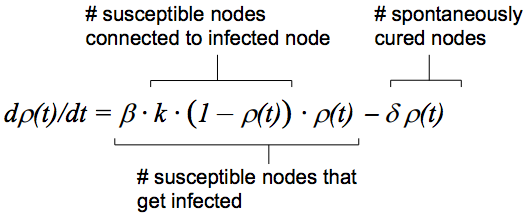
\includegraphics[scale=0.3]{img/SISmodel.png}

        \begin{itemize}
          \item Only two possible states: Susceptible or Infected
          \item $\rho(t)$ fraction of infected nodes
          \item $\beta$: infection rate
          \item $\delta$: cure rate
          \item $k$: number of outgoing edges at each node
        \end{itemize}
  }

  \sectionbox{
    \subsection{Massive Worm examples}
      \begin{itemize}
        \item "Morris" Internet worm (1988)
        \item SQL Slammer, UDP database worm (2003)
        \item Blaster, RPC(=Remote Procedure Call) internet worm (2003)
        \item Sobig.F , Email worm (2003)
        \item Witty worm , "firewall" worm (2004)
       \end{itemize}
  }

  \sectionbox{
    \subsection{Worm Network Impact}
      Primary network impact is due to scanning activity
      \begin{itemize}
        \item ARP flooding
        \item High volume of ICMP destination unreachable msg
        \item Higher network and traffic flows
       \end{itemize}
        \textbf{Network activity anomaly detection:} Entropy measurement of flow header fields. $H = - \sum_{i=1}^{n} p_{i} \log (p_{i})$ ; if $H \leq T $ then raise alert. Determine threshold T using training data.
  }

  \sectionbox{
    \subsection{Malware countermeasures}
     \begin{itemize}
        \item End system: patching, firewall, IPS, Antivirus and educate users (awareness)
        \item Anti-Virus: useful but not too effective
        \item Monocultures are targeted first (e.g. Windows)
        \item Slow patching is a huge risk
        \item Application whitelisting
        \item No trusted intranet
        \item Thin Client (e.g. ChromeOS)
      \end{itemize}
  }

\section{Botnets + Malware Development}
  \sectionbox{
    \textbf{Bot Agent}: crime-ware tool installed on victims\\
    \textbf{Botnet}: collection of all bot agents\\
    \textbf{Bot Master}: the criminal(s) operating the botnet\\
    \textbf{Command and Control}(CnC): botnets management system\\
    \textbf{Opt-in Botnet}: Voluntary botnets (e.g. Low Orbit Ion Cannon)
  }

  \sectionbox{
  \subsection{Objectives to best utilize infected machines}
    \begin{itemize}
      \item \textbf{Buildup} efficient infection and spreading
      \item \textbf{Persistence}: prevent detection and Removal
      \item \textbf{Modularity}: address changing functionality needs
      \item \textbf{Scalability}: handle large number of machines
      \item \textbf{Adaptive}: to business and technology challenges
      \item \textbf{Anonymity}: prevent identification of operator
    \end{itemize}
  }

  \sectionbox{
    \subsection{Target exploitation}
    \begin{itemize}
      \item \textbf{Persist and avoid detection}: explore, steal information, load functionality, maximize yield
      \item \textbf{Move to active attacks}: load attack functionality $\ra$ higher chance of detection
      \item \textbf{Throw away agent}: sell to idiots
    \end{itemize}
  }

  \sectionbox{
  \subsection{Bot Command Modeles}
    \begin{itemize}
      \item \textbf{No Control}: default malicious behaviours, self propagation defaults, less flexible, most likely detected by signatures, most resistant to global shutdown
      \item \textbf{Private Channel}: custom and covert channels, abuse and alteration of common protocols, short-term stealth, signature detection easy once CnC observed
      \item \textbf{Public Infrastructure}: use common applications API, generally reliable and anonymous, mostly IRC, some P2P and microblogging (95\% of today's botnets)
      \item \textbf{Resilient hybrids}: (all models) default malicious behaviors, fall-back plans if CnC unavailable, pre-programmed contact points (drop boxes)
    \end{itemize}
  }

  \sectionbox{
  \subsection{Exploitation Phases}
    \begin{enumerate}
      \item ID Theft (Keylogger, sniffer\ldots)
      \item Peer and Social Attacks (Trust misuse)
      \item Local Attacks (Local Network, USB, VPN)
      \item Attack Support (Host of Phishing Site, Proxying)
      \item External/Noisy Attacks (Scanning, Spam, DDoS)
    \end{enumerate}
  }

  \sectionbox{
  \subsection{Command and Control Topology}
    The ability of a bot agent to locate the CnC infrastructure is a critical requirement for maintaining control of the entire botnet.
    \begin{itemize}
      \item \textbf{Star}: Single centralized CnC (+ Speed of control, - 1 point of failure)
      \item \textbf{Multi-server}: Multiple CnC communicating together (+ No single point of failure, + Geographical optimization, - Advanced planning required)
      \item \textbf{Hierarchical}: Multiple layers below CnC (+ Botnet awareness: single bot agent don't give entire botnet, Ease or resale, - Latency)
      \item \textbf{Random}: No centralized CnC (+ Highly resilient, - Latency,
      - Botnet enumeration)
    \end{itemize}
  }

  \sectionbox{
  \subsection{Fluxing Technologies}
  Botnet takedown attempts typically target the CnC infrastructure
  \begin{itemize}
    \item \textbf{IP-Flux}: Constant change of IP address information related to a particular fully-qualified domain name (FQDN) (cnc.net$\ra$multiple IPs)
    \item \textbf{Domain Flux}: Constant change and allocation of multiple fully-qualified domain names (FQDN) (cnc.net, cnc.ru, abc.net$\ra$ multiple IPs)
    \item \textbf{Single-Flux}: The FQDN of the CnC’s host has multiple IPs addresses assigned (DNS A record)
    \item \textbf{Double-Flux}: The name servers of the CnC’s FQDN as well as the FQDN of the CnC’s host have multiple IP addresses assigned (DNS A and NS records)
  \end{itemize}

  \textbf{Defenders advantage:} Sinkholing: register domain generated by the botnet’s DGAs. "Confickr" generates 50,000 domains per day, and introduced non-determinism in DGA. Taking over all domains costs between \$91.3 million and \$182.5 million per year. Domain registrars are the entity best positioned to mitigate malware that relies on DNS.
  }

  \sectionbox{
  \subsection{Malware Development Process}
    \begin{enumerate}
      \item \textbf{Create} unique samples of malware at \underline{massive scale}
      \item \textbf{Crypter}: encrypt malware to protect against signature detection
      \item \textbf{Protector}: prevent debugging (against reverse engineering, sandboxing)
      \item \textbf{Packers}: make it smaller + use polymorphism
      \item \textbf{Binders}: hide it in another application
      \item \textbf{Quality Assurance}: Test detectability before deployment
    \end{enumerate}
  }

  \sectionbox{
  \subsection{Takedown}
    Legal and technical measures to sever the connection between the CnC structure and the bot agents
  }

  \sectionbox{
  \subsection{Defense}
    \begin{itemize}
      \item Firewalls
      \item Antivirus (up-to-date) but know its limits
      \item Patch your system
      \item brain.exe
    \end{itemize}
  }

% Security Ecosystem and Detection Failures
\section{Security Ecosystem and Detection Failures}

  \emphbox{A vulnerability is a weakness in software (or hardware) that enables an attacker to compromise the software or the data that it processes}

  \sectionbox{
  \subsection{Correlation of Detection Failures}
    Detection failures are \textbf{correlated} – they are not independent events

    The combined failure rate of layered security is typically considerably higher than the product of individual failure rates. $P_{AB} \gg P_{A} \cdot P_{B}$

    Ignoring correlation predicts zero exploits to bypass four or more devices
  }

  \sectionbox{
  \subsection{Security Information Provider}
    \textbf{SIP} = Private and government organizations that \textbf{collect} vulnerabilities, efficiently \textbf{monitor} the primary sources of security information, \textbf{validate} the content found, and \textbf{publish} their findings as security advisories in a consistent format (NVD, CVE). (e.g. CERT, X-Force(IBM), Secunia\ldots)

    \textbf{NVD} = National (USA) Vulnerability Database

    \textbf{CVE} = Common Vulnerabilities and Exposures

    SIPs inform the vendor in order to release a patch $\ra$ average exposure time: 153 days

    When the vendor is not informed about new vulnerabilities $\ra$ average 0-day attack persists: 312 days
  }

  \sectionbox{
    \subsection{Disclosure Options}
    \begin{itemize}
      \item Keep it secret (No disclosure)
      \item Quietly alert vendor
      \item Exploit it by-yourself
      \item Sell on Black Market (Cybercriminals, Governments) between 40k-160k
      \item Sell on White Market (purchase programs: ZeroDayInitiative, VulnerabilityContributorProgram or vendor) $\ra$ Coordinated/Responsible Disclosure (if fails then Full Disclosure)
      \item Full Disclosure
    \end{itemize}
    Choice depends on \textbf{discoverer incentives}: economics, ethics, resources, past experience, publicity, legal constraints
  }

% E-Mail Spam
\section{E-Mail Spam}
  \sectionbox{
  \subsection{Generalities about Spam}
    More than 60\% of email traffic is spam
    \subsubsection{Types of Spam}
      \textbf{UCE}: Unsolicited Commercial Email

      \textbf{UBE}: Unsolicited Bulk Email (not necessarily commercial, sent in masses)

    \subsubsection{Where to get emails addresses}
      \begin{itemize}
        \item Directory Harvest Attack (DHA) against mail server
        \item Email address crawlers
        \item Malware
        \item Harvesting email addresses from databases
      \end{itemize}

    \subsubsection{Spam Sending Tactics}
      \begin{itemize}
        \item Send from borrowed email accounts
        \item Send from short-term officially registered domain
        \item Use fake sender domains
        \item Sending spam from botnet machines
        \item Open mail relays (anyone can do it)
        \item Open proxies
      \end{itemize}

      \subsubsection{Business Models behind Spam}
      \begin{itemize}
        \item Direct sales business: some recipients actually buy spam advertised products; cheap advertising channel; easy to disguise actual sender; hard to enforce anti-spam laws, low risk of getting caught
        \item Internet underground business: operators rent out botnets for sending spam: 1million spam emails sent for 250-700\$ ; 10million email addresses for 100euros
      \end{itemize}
      }
  }

  \sectionbox{
  \subsection{Anti-Spam Techniques}
    \begin{itemize}
      \item \textbf{Filter at SMTP time}: +cheap and fast -lack info. to decide
      \item \textbf{Whitelists}: allow only emails matching non spam criteria
      \item \textbf{Greylists}: defer 1st email but accept follow-up email (issues with delays and multiple SMTP hosts of larger hosters)
      \item \textbf{Blacklists}: reject email matching spam criteria
        \begin{itemize}
          \item DNS Blacklisting: can be done either with IP or domain name.   URL which redirects to another URL $\ra$ defeats Blacklists.
          \item Blacklists caveats: evasion (botnet,stolen email, short term unpaid domains), denial of service (email on list don't work anymore$\ra$blacklists operators have power)
        \end{itemize}
      \item \textbf{Filtering SMTP traffic at FW}: block outgoing SMTP msg not from SMTP server (prevent email-based worms)
      \item \textbf{Heuristical Content Filtering}: look at weird font, strange URL \ldots)
      \item \textbf{Statistical Content Filtering}:\\
      $P(spam|words) = \frac{P(words|spam)P(spam)}{P(words)}$

      Misspellings in text $\ra$ defeats Naive Bayesian filter.
      \item \textbf{Traffic Based Filtering}: Compare flux of emails to recognize bulk mail (DCC = Distributed Checksum Clearinghouse)
      \item \textbf{Image Spam Filtering}: OCR on images before filtering
      \item \textbf{Text Filtering Caveats}: Normalize content before filtering text
    \end{itemize}
  }

\sectionbox{
 \subsection{Spam fighting at ETH}
  Bayesian filter not used (broad range of messages at University)

   Running parallel SMTP sessions with filtering processes : this is a best effort service.
   They reject confirmed spam email directly. They keep in a “phish trap” suspected spam.
   They provide tag-only option for spam, and personal blacklist/whitelist

   \textbf{Phishing Countermeasures:} (other than Phish trap)
   \begin{itemize}
     \item Set a daily limit on the number of messages that can be sent by a user
     \item Lock accounts sending spam/phish/malware messages or hosting a phishing web page
     \item Inform phishing recipients that their account may be “phished”
     \item Remove phishing messages from user mailboxes
     \item Redirect a phishing URL to a warning web page OR Block a phishing URL’s IP-address
   \end{itemize}
   \textbf{ETH is keeping logs for one year:} sender-host/IP; sender/recipient address; subject header (40 characters); attachment file name; delivery/rejection status

   \textbf{For:} filter modifications - check for false positives/negatives; message tracking; data mining - identify botnet members, etc.; statistics
 }

  \sectionbox{
  \subsection{Email Authentication}
    \begin{itemize}
      \item \textbf{S/MIME}(Secure/MIME): sign and encrypt only msg content (not header)
      \item \textbf{PGP}(Pretty Good Privacy): auth + encry with Web of Trust
      \item \textbf{DKIM}(DomainKeys Identified Mail): Sign mails between servers
      \item \textbf{SPF}(Sender Policy Framework): List of IPs allowed to send emails
      \item \textbf{SenderID}: Match PRA domain against source IP via DNS (PRA is often From: header)
    \end{itemize}

    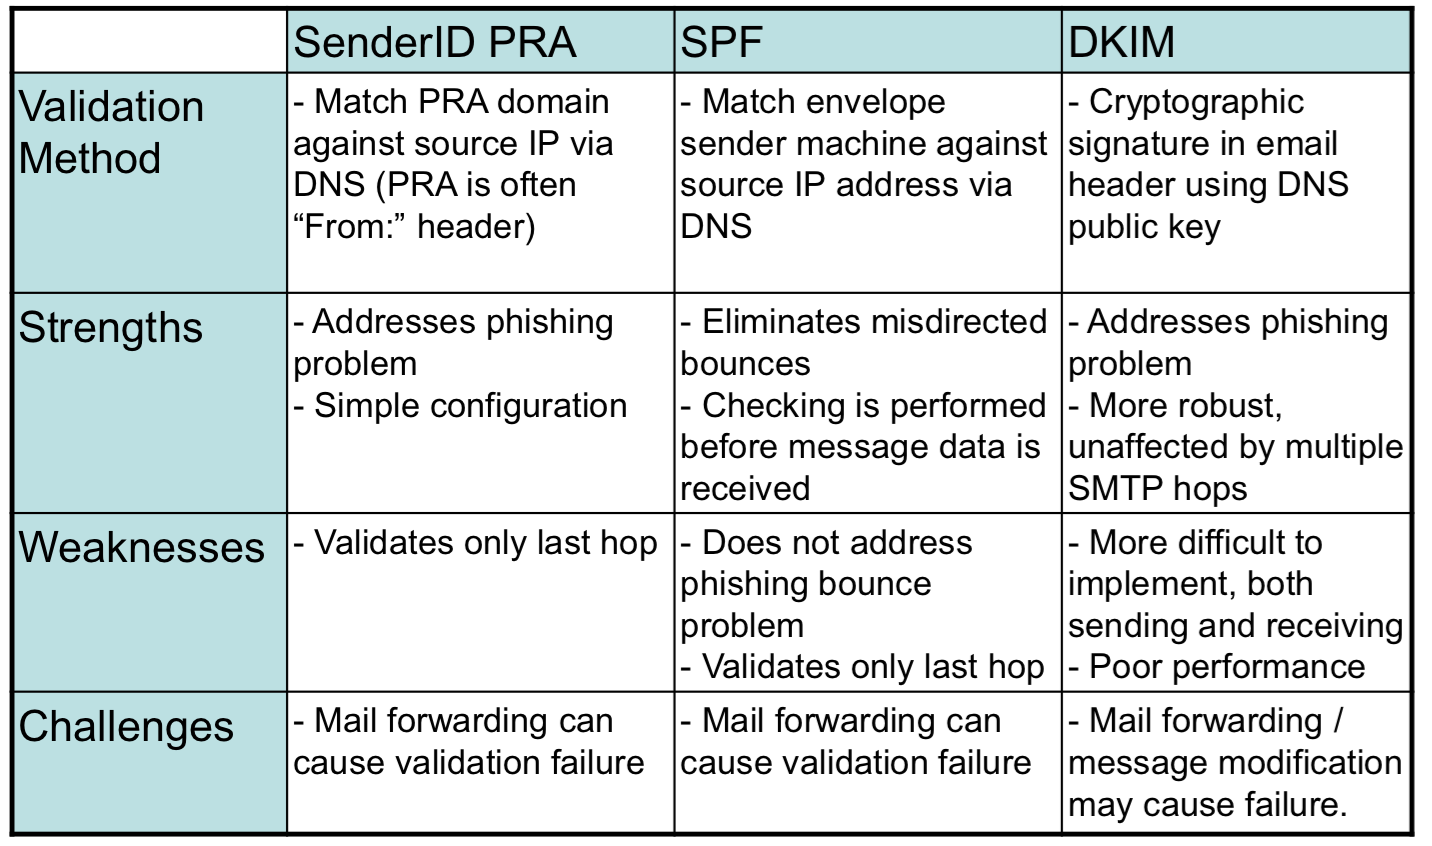
\includegraphics[width=\columnwidth]{img/emailauth.png}
  }

\section{Guest Lectures}
  \sectionbox {
  \subsection{Trusted Computing by Swisscom}
    Trust is based on 3 conditions
    \begin{enumerate}
      \item \textbf{Positive Intention} (always positive intentions)
      \item \textbf{Transparency and predictability}
      \item \textbf{Reliability and continuity} (long strong trust)
    \end{enumerate}

    Need to secure hardware first to have secure software :
    \begin{enumerate}
      \item Vendor Flash (MicroCode) initialize TPM
      \item Microcode initiate boot sequence of Firmware
      \item During boot time BIOS + tboot log every steps in TPM + hash it
      \item Boot sequence reported during secure boot sent to attestation server
      \item Attestation server checks with previously recorded reference values
      \item Integrity confirmed or rejected (contact Whitelist server)
      \item Integrity checked; boot or stop ($\simeq$3 minutes)
    \end{enumerate}

    \begin{itemize}
      \item \textbf{TPM}: Trusted Platform Module
      \item \textbf{TEE}: Trusted Execution Environment (e.g. Trust Zone)
      \item \textbf{TXT}: Trusted Execution Technology (SecureBoot)
      \item \textbf{SE}: Secure Elements (e.g. SIM- Card MobileID)
      \item \textbf{CIT}: Cloud Integrity Technology
    \end{itemize}
  }

  \sectionbox {
  \subsection{Air Traffic Control by ArmaSuisse}
      Current Air Traffic Control use 2 systems synchronized:
      \begin{itemize}
        \item \textbf{PSR}(Primary Surveillance Radar): Independent surveillance made with ground based radar
        \item \textbf{SSR}(Secondary Surveillance Radar): Dependance surveillance using transponder-based interrogation
      \end{itemize}

      \underline{Problems}: high cost, low accuracy

      Future Air Traffic Control $\ra$ \textbf{ADS-B}
      \begin{itemize}
        \item \textbf{A}utomatic: Always on (no explicit interrogation)
        \item \textbf{D}ependent: On-board system provides info to other parties
        \item \textbf{S}urveillance: Precise info (altitude, ID, speed)
        \item \textbf{B}roadcast: Send to everyone equipped to receive the data
      \end{itemize}

      \underline{Problems}: No CIA(A), assume everything can be trusted
      \begin{itemize}
        \item Eavesdropping: cheap hardware and not encryption (flightradar24.com)
        \item Active attacks: message injection/deletion/modification
          \begin{itemize}
            \item Ghost Aircraft Flooding $\ra$ DOS on surveillance system
            \item Virtual Trajectory Modification
            \item \ldots
          \end{itemize}
      \end{itemize}

      \underline{Solutions}: Large Sensor Deployment to check, \ldots
      \begin{itemize}
        \item Time Difference of Arrival (TDoA) $\Ra$ Position validation
        \item Secure Track Verification (No need for tight time synchronisation)
      \end{itemize}
  }

  \sectionbox{
  \subsection{Fighting Cybercrime as a CERT by SWITCH}
    \textbf{SWITCH} = non-profit foundation of Swiss Universities, ISP for Universities + in charge of the .ch + monitors flows to detect bots in Switzerland and fake .ch website (usually hosted outside of Switzerland)

    \textbf{CERT}(Computer Emergency Response Team) = support, protect and prevent, internationally networked

    \textbf{Retefe Malware} = Banking Trojan targeting CHE, SWE and JPN
    \begin{enumerate}
      \item Executable in an email installs a new root certificate + reconfigure proxy to re-route traffic for targeted banking websites.
      \item When the victim try to reach his bank's website, the malicious DNS server returns the IP address of a rogue web-server containing a copy of the website.
      \item No certificate warning from browser because of fake root certificate.
      \item Victim types in his username, password and send it to the attacker through the fake website.
      \item Then fake website propose to install a smartphone app to be able to forward the bank's mTan to the attacker.
      \item Attacker has full control and use another compromised PC in the geographical area as a proxy to connect to the bank account of the victim.
    \end{enumerate}

    %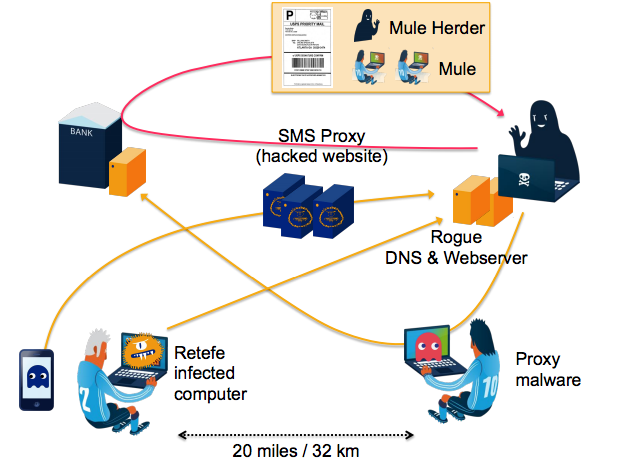
\includegraphics[width=\columnwidth]{img/Retefe-Malware.png}

    \textbf{Carbanak Cybergang} stole \$1bn from 100 banks directly. Malware install on admin computer (targeted attacks). Attackers spies on them to learn how to use the specific money transfer software of each bank.
  }

  \sectionbox{
  \subsection{Malware Analysis and Prevention by Symantec}
    \textbf{The 3 Main Attack Vectors}:
    \begin{enumerate}
      \item \textbf{Spear Phishing}: Email with link or malicious attachment
      \item \textbf{Drive-by download attack}: Website uses an exploit to drop malware
      \item \textbf{Supply-chain hack}: Compromise vendors and supplier software
    \end{enumerate}
	  \textbf{Malware analysis procedure}
	  \begin{enumerate}
  	  \item Get a sample from customers, traps, crawlers\ldots
  	  \item Automated analysis (VirusTotal.com, ThreatExpert\ldots)
  	  \item Blackboxing(Sandboxing): monitor all operating system calls (behavior)
  	  \item Whiteboxing: Disassembling/debugging code to understand it $\ra$ need to bypass code obfuscation and understand the domain generation algorithm (DGA)
  	  \item write description of the threat and create a signature to block it
  	  \item start again (The analysis hamster wheel)
	  \end{enumerate}
  }

  \sectionbox{
    \subsection{SCION Secure Next-Generation Internet Architecture}
    SCION is an isolation architecture only for the control plane, in the data plane it is a transparency architecture.
    \subsubsection{Isolation Domain (ISD)}
    Region that can agree on a common root of trust $\Ra$ authenticate entities only within each ISD (e.g. domain on geographical regions) political and legal issues arise

    \subsubsection{SCION Architectural Design Goals}
    \begin{itemize}
        \item High availability, even for networks with malicious parties
        \item Adversary: access to management plane of router
        \item Communication should be available if adversary-free path exists
        \item Secure entity authentication that scales to global heterogeneous (dis)trusted environment
        \item Flexible trust: operate in heterogeneous trust environment
        \item Transparent operation: Clear what is happening to packets and whom needs to be relied upon for operation $\Ra$ \textbf{Packet-Carried State:} Packets carrying forwarding information
        \item Balanced control among ISPs, Senders, and Receiver
        \item Scalability, efficiency, flexibility
    \end{itemize}
    \textbf{Beaconing for Route Discovery:} Scalable and secure dissemination of path/topological information from core to edge. Policy-constrained multi-path flood to provide multiple paths.

    \subsubsection{SCION Dangers}
    \begin{itemize}
        \item Too many top-level ISDs , ISPs part of ISD core
        \item Large packet header size
        \item Too many extensions used
        \item Higher complexity (Extensions, PKI)
        \item Extremely high path fluctuations, changes
      \end{itemize}
    }

    % \section{Hacking labs}
    % \sectionbox{
    % \subsection{Tools}
    % \begin{itemize}
    %     \item \textit{nslookup website.ch} : Generate DNS traffic
    %     \item to check ARP table : \textit{arp -a} $\Ra$ ARP is a layer 2 protocol
    %     \item \textbf{Wireshark} : GUI tool to capture traffic
    %     \item \textbf{Tshark} is a command line tool like tcpdump. Command line tools are more reliable than GUI tools because it might happen that your CPU gets overloaded and some packets have to be dropped.
    %
    %     Use the following command to capture HTTP traffic on the interface 2: \textit{tshark -i 2 -f "port 80" -w output.pcap}
    %     \item \textbf{Nmap or Fingerprinting}
    %     Used to find vulnerable targets and services.
    %
    %     \textit{nmap -O -oX nmap\_result.xml -sV - -reason targetIP}
    %
    %     -O : This is an operating system scan.
    %
    %     -oX : Output the scan to an XML file.
    %
    %     -sV: Tests open ports to determine the listened service and its version
    %
    %     - -reason: Give the reason for the apparent state of a port.
    %     \item \textbf{Scapy} is a powerful interactive packet manipulation program. It is able to forge or decode packets of a wide number of protocols, send them on the wire, capture them, match requests and replies, and much more. It can easily handle most classical tasks like scanning, tracerouting, probing, unit tests, attacks or network discovery.
    %     \item \textbf{Metasploit} : penetration testing tool. It simulates real-world attacks to find weak points before a malicious attacker does.
    %     \item \textbf{XSS Shell} = XSS backdoor and zombie manager $\ra$ can interactively send requests and get responses from victim ($\simeq$ backdoor the page)
    % \end{itemize}
    % }
    %
    % \sectionbox{
    % \subsection{Worm Conficker Attack}
    %  computer worm targeting the Microsoft Windows operating system that was first detected in November 2008. It uses flaws in Windows OS software and dictionary attacks on administrator passwords to propagate while forming a botnet, and has been unusually difficult to counter because of its combined use of many advanced malware techniques.
    % }
    %
    % \sectionbox{
    % \subsection{Session Fixation}
    %   the victim is fixing the session for the attacker.
    %   Most session fixation attacks are web based and most rely on session identifiers being accepted from URLs (query string) or POST data. Session-Fixation is related to Session-Hijacking. The attacker will send his victim a link with a valid web application session (asked from the webApp) appended. Through social engineering, a trustful victim will click on the link and provide credentials.
    % }


\end{document}
